\chapter{Building materials models}\label{ch:advanced}

\chapterlead{Crystal defects, molecules on surfaces, and polymer mixtures can all be built step by step from a small set of well-defined structural inputs. This chapter explains how to choose those inputs, interpret construction parameters, and check the resulting models. Each example aims to produce a suitable initial structure with a clear provenance for subsequent calculations.}

\section{Build a crystal from a space group}
\index{Space groups}

\subsection{Understand asymmetric sites}

Many atomic positions in a crystal are related by symmetry. A space-group construction therefore needs only a lattice, space group, and asymmetric sites, rather than every atom individually. The tool expands their equivalent positions. Understanding that the input is asymmetric sites and the output is a complete working cell is central to using the crystal builder.

Specify the space group by symbol or number. \ui{Lattice matrix} is an editable $3\times3$ table: rows a, b, and c are the lattice vectors; columns x, y, and z are their Cartesian components in \AA. Click and edit individual cells. Each asymmetric site also requires an element, fractional coordinates, and occupancy. Occupancy 1 means full occupancy by that element. Partial occupancy describes an average structure; calculations requiring explicit atomic arrangements generally need an ordered approximation or alloy model.

\subsection{Example: face-centered cubic copper}

Build a conventional face-centered cubic Cu cell with $a=3.61\,\text{\AA}$. This is an example input; replace it with appropriate experimental or calculated data for your work.

\begin{steps}
  \item Open and activate a crystal document from the \ui{Project Browser}. On \ui{Crystal Modeling}, open \ui{Symmetry Tools} in \ui{Crystal \& Cell}, then choose \ui{Build from Space Group}.
  \item Enter \file{Fm-3m} under \ui{Space-group symbol or number}. In \ui{Lattice matrix}, set the a/x, b/y, and c/z diagonal cells to 3.61 and the other six cells to 0.
  \item Enter Cu under \ui{Element symbol} and \literalinput{0 0 0} in the \ui{Asymmetric fractional coordinates} text field. Set \ui{Asymmetric-site occupancies} to 1 and initially retain the expanded-position overlap tolerance of $0.1\,\text{\AA}$.
  \item Preview and inspect the expansion. A conventional face-centered cubic cell should contain 4 Cu sites, rather than only the one input position.
  \item Click \ui{Apply}. In the result window, inspect asymmetric and equivalent site information, check elements, occupancies, and positions, then save as \file{Cu-fcc}.
\end{steps}

Only one asymmetric site is needed; the space group generates the other positions. If expanded sites collide, first check whether equivalent positions have been entered more than once, rather than immediately reducing the collision tolerance. Supplying a site already generated by the space group as another independent input can duplicate the same atom.

The supplied \file{Cu-fcc.cif} is the four-site cell generated with these settings. \file{Cu-vacancy.cif} is one result of the later vacancy enumeration and contains three sites. The accompanying script regenerates both structures.

\subsection{Choose a cell representation}

A primitive cell uses fewer atoms to represent translational periodicity. A conventional cell often makes symmetry and crystal axes clearer. Different shapes and atom counts for the same material do not imply a composition change. Compare formula, volume, and site count together rather than judging only the displayed cell size.

\ui{Symmetry}, \ui{Primitive Cell}, and \ui{Conventional Cell} use positional and angular tolerances. Their defaults are $0.01\,\text{\AA}$ and $5^\circ$. These determine whether slightly displaced positions are still treated as symmetry equivalent. A large tolerance may interpret a real distortion as numerical noise, so assess the result in light of the model's origin.

\ui{Make P1} explicitly retains the current atoms without additional declared space-group constraints, which is useful for local editing. Atomic positions and their geometric symmetry are preserved; subsequent edits no longer depend on the original space-group declaration.

\section{Adjust the cell}

\subsection{Choose the right cell operation}
\index{Strain}

\ui{Edit Lattice} lets you choose whether to preserve Cartesian atomic positions. \ui{Redefine Lattice} preserves them while changing the lattice that encloses them. Both dialogs edit a table with lattice vectors in rows a, b, c and Cartesian components in columns x, y, z. \ui{Strain Structure} instead applies a homogeneous deformation to the entire structure. Decide whether your goal is to change the boundary description or to scale internal distances with the lattice.

For example, entering \file{0.01} under \ui{Strain} applies engineering strain 0.01 in all three directions, multiplying lengths by 1.01 rather than adding $0.01\,\text{\AA}$. To stretch only the first direction, enter \literalinput{0.01 0 0} in the same field. Preview, inspect lattice lengths, angles, and local distances, then save.

\ui{Orthogonalize Cell} searches integer supercells subject to length, angle, and atom-count limits. It can prepare an approximately orthogonal box for later processing, but not every lattice has an exact orthogonal representation within a finite search range. If no result is found, consider increasing the maximum length or atom count, or relaxing the angular tolerance where appropriate. Larger supercells also increase subsequent calculation costs.

\section{Screen defect configurations}
\index{Defect enumeration}

Creating the same defect at symmetry-related sites can produce equivalent models. \ui{Enumerate Point Defects} combines such duplicates and reports their degeneracy: the number of positions belonging to the same class. Degeneracy does not rank defect energies.

\begin{steps}
  \item Open the earlier \file{Cu-fcc} model and choose \ui{Enumerate Point Defects}.
  \item Set the defect type to \file{vacancy}, using the Cu cell's sites as candidates. Retain the default positional and angular tolerances initially.
  \item Click \ui{Apply} and inspect the candidate table. The four sites in ideal conventional face-centered cubic Cu are equivalent, so there should be one vacancy candidate with degeneracy 4.
  \item Check its remaining atom count, composition, and contacts. Open the added defect structure from the Project Browser and save the project, retaining both pristine copper and the defect result.
\end{steps}

A substitution requires the replacement element; an interstitial requires the new atom's coordinates and coordinate type; an antisite exchanges elements between sites. Similar names describe different structural changes. Check element counts first, then positions, to catch input mistakes more easily than by inspecting the image alone.

\ui{Generate SQS Model} converts partial occupancies or mixed compositions into explicit arrangements in a finite cell. The tool enumerates or performs a time-limited search against pair-correlation targets, with configurable supercell scaling and search budget. The budget affects candidate quality and elapsed time. Retain the model together with its composition, cell size, and search settings for comparison.

\section{Example: build a \headinglatin{Pt}(111) surface}
\index{Surface models}

\subsection{Understand a slab model}

A surface model usually consists of a finite crystal slab and vacuum. It repeats periodically in-plane, while vacuum separates neighboring slabs along the normal. Miller indices $(hkl)$ specify the cut plane. Slab thickness, termination, and vacuum together define the resulting model.

\subsubsection{Obtain the normal from Miller indices}

A crystal plane's normal is determined by reciprocal vectors. Using the convention in Chapter~\ref{ch:theory},
\begin{equation}
  \mathbf G_{hkl}=h\mathbf b_1+k\mathbf b_2+l\mathbf b_3,
  \qquad
  \hat{\mathbf n}=\frac{\mathbf G_{hkl}}{\|\mathbf G_{hkl}\|}.
  \label{eq:surface-miller-normal}
\end{equation}
The reciprocal vectors $\mathbf b_1,\mathbf b_2,\mathbf b_3$ have units $\text{\AA}^{-1}$; $h,k,l$ are dimensionless integers and $\hat{\mathbf n}$ is a unit normal. In a cubic cell, the (111) normal is parallel to $\mathbf a+\mathbf b+\mathbf c$. Here the lattice axes align with global axes, so it is also parallel to global $(1,1,1)$. A skewed cell generally lacks this correspondence: do not use Miller indices directly as a Cartesian adsorbate-orientation vector.

For a constructed slab with in-plane vectors $\mathbf a,\mathbf b$, check its actual normal and cell height using
\begin{equation}
  \hat{\mathbf n}_{\mathrm{slab}}=
  \frac{\mathbf a\times\mathbf b}{\|\mathbf a\times\mathbf b\|},
  \qquad H=|\mathbf c\cdot\hat{\mathbf n}_{\mathrm{slab}}|
  \label{eq:surface-normal-height}
\end{equation}
The height $H$ is the repeat distance between periodic slabs along the normal, and need not equal $\|\mathbf c\|$. First choose periodic images that form one continuous slab, then project the atomic positions onto the normal to measure the distance between the outermost layers. Record this distance separately from the requested minimum thickness and the thickness of the complete structural repeats used for construction.

\begin{table}[H]
\centering
\caption{Lengths used in surface construction.}
\begin{tabularx}{\linewidth}{lX}
\toprule
Quantity & Interpretation and checks\\
\midrule
Minimum slab thickness & A criterion for selecting complete repeat units, not a direct layer count.\\
Atomic-layer span & Normal distance between outermost layers; select one continuous slab first.\\
Cell height $H$ & Measured along the surface normal, Eq.~\eqref{eq:surface-normal-height}; includes the slab and periodic gap.\\
Added vacuum $\Delta$ & Length added along the third lattice vector by \ui{Add Vacuum}, not the final total vacuum.\\
\bottomrule
\end{tabularx}
\end{table}

For nonorthogonal input, also check the output normal, layer count, and periodic separation. Orientation handling can affect thickness conversion and candidate reduction; the minimum input thickness alone does not establish the result. The platinum example starts from a cubic cell and checks the generated slab.


A minimum slab thickness is not an exact number of atomic layers. The builder selects complete structural repeats to preserve stacking, and different planes and terminations can give different atom counts. After entering $8\,\text{\AA}$, inspect the layer count in the generated model.

First build bulk Pt with \ui{Build from Space Group}. Enter \file{Fm-3m}. Set the a/x, b/y, and c/z cells of \ui{Lattice matrix} to 3.92 and the other six cells to 0, giving a cubic lattice with side length $3.92\,\text{\AA}$. Enter Pt under \ui{Element symbol}, \literalinput{0 0 0} under \ui{Asymmetric fractional coordinates}, and 1 under \ui{Asymmetric-site occupancies}. Preview and inspect the bulk cell before generating its (111) surface.

\begin{table}[htbp]
\centering
\caption{Parameters for the Pt(111) surface exercise.}
\begin{tabularx}{\linewidth}{lX}
\toprule
Parameter & Setting and meaning \\
\midrule
Miller indices (h k l) & Enter 1, 1, 1 in the three fields to select (111).\\
Minimum slab thickness & $8\,\text{\AA}$; check the generated layers and geometric thickness.\\
Minimum vacuum & $10\,\text{\AA}$ for this construction exercise.\\
Center slab & Enabled, placing the slab centrally along the cell normal.\\
Primitive surface cell & Enabled, using the corresponding reduced surface repeat.\\
Termination index & 1; compare terminations separately if several are available.\\
\bottomrule
\end{tabularx}
\end{table}

\begin{steps}
  \item Activate bulk Pt. On \ui{Crystal Modeling}, open \ui{Surface Modeling} in \ui{Surfaces \& Interfaces}, then choose \ui{Build Slab}.
  \item Enter the table's values and preview. Inspect the in-plane arrangement nearly along the normal, then turn to the side to inspect thickness and vacuum.
  \item Set the termination index to 1. After applying, inspect termination information in the result window, considering surface elements, stacking, and your research objective.
  \item Check the atoms against the cell boundary, record the actual atom and layer counts, and save as \file{Pt111-slab}. To try another termination, return to bulk Pt, reopen the command, and change the termination index. The candidate table is for inspection only.
\end{steps}

% Native English captures; see docs/provenance/english-edition-assets.json for source and crop metadata.
\begin{figure}[H]
\centering
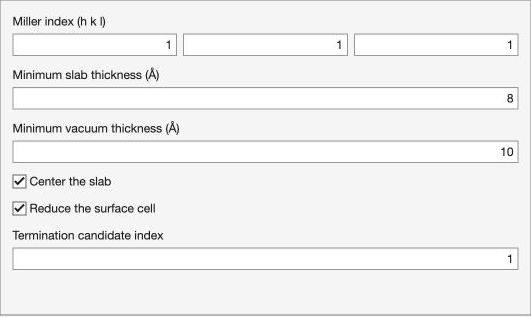
\includegraphics[width=107mm]{publication-assets/crop-e2fa9f70b6bcca245a04.png}
\par\vspace{2mm}
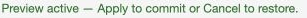
\includegraphics[width=80mm]{publication-assets/crop-f2ece60af591133fac37.png}
\caption{Pt(111) construction after importing \file{Pt-fcc.cif}: Miller indices 1, 1, 1; minimum slab thickness $8\,\text{\AA}$; minimum vacuum $10\,\text{\AA}$; centering and primitive surface cell enabled; termination candidate 1. The preview message appears below.}
\label{fig:pt111-slab-parameters}
\end{figure}


The supplied \file{Pt-fcc.cif} and \file{Pt111-slab.cif} contain the bulk and slab models. These parameters give 4 independent sites in 4 geometric layers. Along the normal, the cell's periodic height is approximately $20.3689\,\text{\AA}$, the outermost atomic planes span approximately $6.7896\,\text{\AA}$, and the separation between outermost planes of neighboring periodic slabs is approximately $13.5793\,\text{\AA}$. The thickness used for construction is based on complete crystal repeats and differs from the distance between the outermost atomic planes. Project distances along the normal; the third vector's length in an oblique cell is not directly the vacuum thickness.

\subsection{Fix the bottom layers}
\index{Fixed atoms}
\index{Vacuum}

Surface relaxations often hold some bottom layers fixed to approximate the constraint from deeper bulk material. After slab construction, the tool can identify geometric layers. Open \ui{Fix Atoms} and set the bottom-layer count to 1 to select the lowest layer. To use an explicit selection instead, set the bottom-layer count to 0 as directed by the interface and select the intended sites.

Fixed flags are stored in the model. Enable the required constraints in the relevant calculation task when submitting it. Thicker slabs may need several fixed layers. Begin with one and inspect its extent to understand the setting.

\subsection{Add vacuum}

\ui{Add Vacuum} increases space along the third lattice vector; the input is an additional thickness. If that vector is inclined to the surface normal, the added normal projection is smaller than the entered length. Here the exercise uses a cell with its third vector along the normal. Adding $5\,\text{\AA}$ adds to the existing model rather than setting total vacuum to $5\,\text{\AA}$. Check the cell and slab from the side after applying. Adsorbates or solvent can occupy some previously empty space, so inspect the complete model again after adding them.

Adding vacuum changes the geometry according to
\begin{equation}
  \mathbf c'=
  \frac{\|\mathbf c\|+\Delta}{\|\mathbf c\|}\,\mathbf c,
  \qquad
  \Delta H=\Delta\,
  \left|\frac{\mathbf c}{\|\mathbf c\|}\cdot\hat{\mathbf n}_{\mathrm{slab}}\right|.
  \label{eq:vacuum-addition-projection}
\end{equation}
Both $\Delta$ and $\Delta H$ are in \AA. The former is the requested added length; the latter is the increase in cell height measured perpendicular to the slab. The dot-product factor lies between 0 and 1. With $\mathbf c$ along global $z$ and the surface normal along $(1,1,1)$, adding $2\,\text{\AA}$ increases this perpendicular height by only approximately $2/\sqrt{3}=1.155\,\text{\AA}$. In Figure~\ref{fig:surface-vacuum-geometry}, $\Delta\mathbf c=\mathbf c'-\mathbf c$ has length $\Delta$, and $\Delta H$ is the length of its projection onto the surface normal. Aligning $\mathbf c$ with the normal first makes the added length equal to the increase in the gap between periodic slabs.


\begin{steps}
  \item Import \file{Pt111-normal-c.json} afresh, retaining an unmodified slab. Its third vector already follows the surface normal. Open \ui{Add Vacuum} under \ui{Surface Modeling} on \ui{Crystal Modeling}.
  \item Set additional thickness to $5\,\text{\AA}$. Preview and compare the slab with the cell boundary from the side, confirming that the extra space lies outside the slab.
  \item Apply and recheck Pt site count and internal geometry. Adding vacuum should neither add Pt atoms nor increase the slab's internal layer spacing.
  \item Save as \file{Pt111-extra-vacuum}, separately from the original slab. Restart later adsorption exercises from their specified original files.
\end{steps}

\begin{figure}[H]
\centering
\begin{tikzpicture}[x=1mm,y=1mm,font=\sffamily\small,>=stealth]
  \foreach \shift in {0,65} {
    \fill[paleblue] (\shift+12,15) rectangle (\shift+44,25);
    \draw[teal] (\shift+12,15) -- (\shift+44,15);
    \draw[teal] (\shift+12,25) -- (\shift+44,25);
    \foreach \x in {16,25,34,43} {
      \fill[brand] (\shift+\x,18) circle (1.3);
      \fill[teal] (\shift+\x-2,22) circle (1.3);
    }
    \draw[->,brand,line width=.7pt] (\shift+12,6) -- (\shift+45,6)
      node[right] {$\mathbf a$};
    \draw[densely dashed,muted] (\shift+12,25) -- (\shift+12,53);
  }
  \node[text=brand] at (29,65) {Oblique third vector};
  \node[text=brand] at (94,65) {Third vector along normal};
  \draw[->,brand,line width=.8pt] (12,6) -- (34,44)
    node[pos=.55,right] {$\mathbf c$};
  \draw[->,teal,line width=1pt] (34,44) -- (41,56)
    node[pos=.6,right] {$\Delta\mathbf c$};
  \draw[densely dashed,muted] (34,44) -- (51,44);
  \draw[densely dashed,muted] (41,56) -- (51,56);
  \draw[<->,teal] (49,44) -- (49,56);
  \node[anchor=south,text=teal,font=\sffamily\footnotesize] at (48,57) {$\Delta H$};
  \draw[->,muted,line width=.7pt] (6,28) -- (6,49)
    node[above] {$\hat{\mathbf n}$};
  \draw[->,brand,line width=.8pt] (77,6) -- (77,44)
    node[pos=.52,left] {$\mathbf c$};
  \draw[->,teal,line width=1pt] (77,44) -- (77,56)
    node[right] {$\Delta H=\Delta$};
  \node[align=center,font=\sffamily\footnotesize] at (29,-4)
    {Normal increase is smaller\\than the added length along $\mathbf c$};
  \node[align=center,font=\sffamily\footnotesize] at (94,-4)
    {Added length equals\\the normal increase};
\end{tikzpicture}
\caption{Directions when adding vacuum (section schematic). Relative positions within the slab remain fixed as the third lattice vector extends along its original direction and the slab is recentered. Only a vector normal to the surface converts the full added length into normal separation.}
\label{fig:surface-vacuum-geometry}
\end{figure}


\section{Place adsorbates on a surface}
\index{Adsorption modeling}

\subsection{Choose an adsorption site}

Adsorption modeling must specify where to place a molecule, which atom anchors it, and its orientation. An ontop site lies above a surface atom, a bridge site between two atoms, and a hollow site within a region enclosed by several surface atoms. The anchor atom determines which molecular atom is placed at the specified height; an orientation atom helps define its direction.

Use \ui{Find Adsorption Sites} to relate candidate positions to the surface. The default height is $2\,\text{\AA}$. Sites are geometric references for initial configurations, not evidence of stable adsorption.

\subsection{Prepare the adsorption cell}

Import an unmodified \file{Pt111-slab.cif}; do not use the version with extra vacuum from the previous section. Its surface normal follows global $(1,1,1)$, while the original $c$ vector follows global $z$. The current parameter command adds anchor height along $c$. Aligning $c$ with the normal first makes the entered height agree with the vertical distance in the side view.

Open \ui{Redefine Lattice}, retain rows $a$ and $b$, and set the $x$, $y$, and $z$ components of row $c$ to 11.76, 11.76, and 11.76 in \AA, preserving Cartesian positions. This uses $c_{\mathrm{new}}=c+6a+6b$ without building a supercell, so there are still 4 Pt sites. The new $c$ is perpendicular to the surface; the in-plane angle between $a$ and $b$ remains $60^\circ$. Alternatively, import the prepared \file{Pt111-normal-c.json}.

Inspect the slab and cell boundary from the side. Vector $c$ should point outward normal to the surface, with internal layer positions unchanged. For another surface, determine its normal from the in-plane vectors rather than copying these components.

\subsection{Example: place an \headinglatin{O--H} fragment interactively}

Interactive placement lets you see how a molecule approaches the surface while adjusting the complete fragment's height, orientation, and contacts.

\begin{steps}
  \item Open the prepared \file{Pt111-normal-c}. Press O to enter adsorbate placement and choose O--H. The fragment toolbar can also use project molecules or user fragments.
  \item Drag outward from a surface atom to establish the relationship between the surface site and fragment anchor. Adjust the view so the drag direction is clear.
  \item Drag with the left button to change the fragment's orientation, Alt+left-drag to change anchor distance, and right-drag to rotate about the anchoring direction.
  \item Check that O--H connectivity is retained and that the fragment is not too close to nearby surface atoms. Press Enter or \ui{Apply} when the preview is suitable.
  \item Save a separate adsorption model. Undo and place it again if another approach is needed.
\end{steps}

\subsection{Example: place \headinglatin{O--H} outward using parameters}

Parameter-based placement makes configurations easy to record and reproduce. The supplied \file{oh-fragment.mol} contains O and H joined by one single bond of length $0.96\,\text{\AA}$. Import it into the project, then import and activate a fresh \file{Pt111-normal-c.json} to start from a clean four-site host.

\begin{steps}
  \item Open \ui{Place Adsorbate} and select the imported O--H molecule under \ui{Project adsorbate}.
  \item Choose ontop, candidate index 1, and \ui{Anchor height (Å)} of 2.
  \item Set anchor atom to 1 (O) and orientation atom to 2 (H). Enter 1, 1, 1 in the direction fields so the O-to-H direction follows this surface normal. Retain the minimum allowed distance of $0.5\,\text{\AA}$.
  \item Preview from the side: O should lie above the selected Pt atom, with H farther from the surface. Then click \ui{Apply}.
  \item This input has negative fractional coordinates. To view host and adsorbate within one unit cell, open \ui{Build Supercell}, enter 1 in all three scaling components, and apply. This wraps equivalent sites into the unit cell without enlarging the model. The lattice and 6 independent sites remain unchanged.
  \item Rename the result \file{Pt111-OH-outward} and save. Display the cell boundary and inspect the O--H direction from the side. Boundary images may show the same fragment several times; check composition against the 6 independent sites in the summary.
\end{steps}

% Native English captures; see docs/provenance/english-edition-assets.json for source and crop metadata.
\begin{figure}[H]
\centering
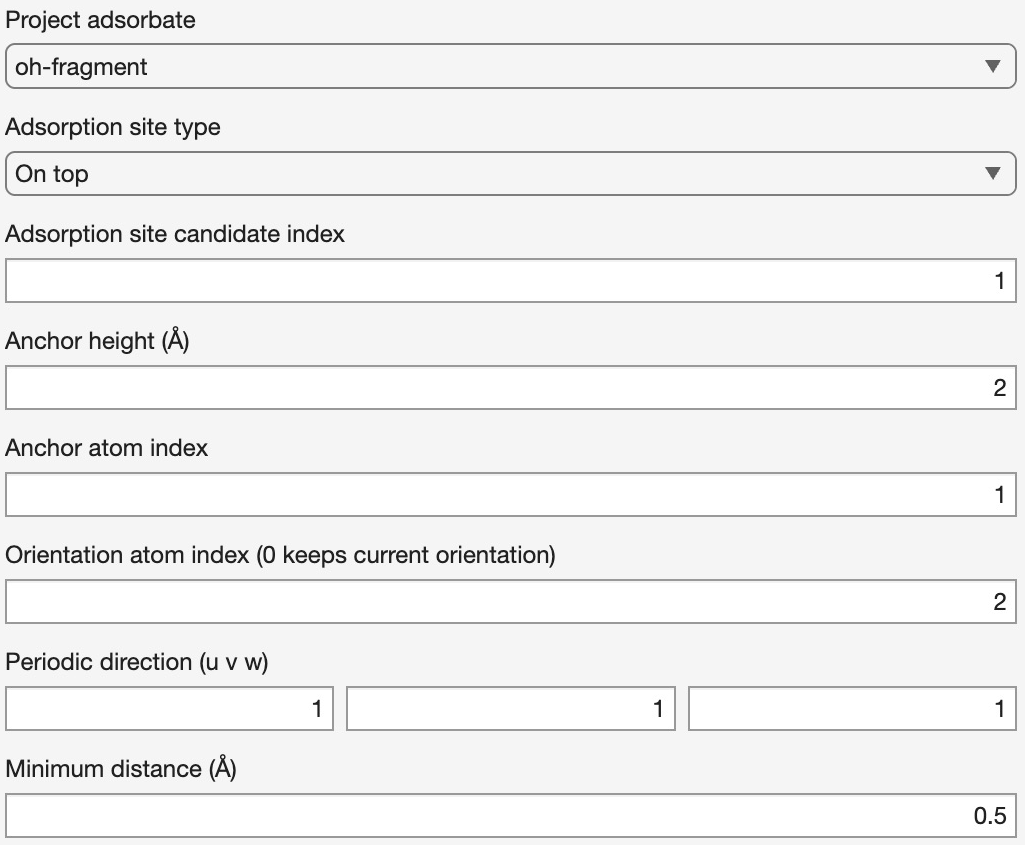
\includegraphics[width=107mm]{publication-assets/crop-c02e14aa8762e8947bbe.png}
\caption{Outward O--H placement: project fragment \file{oh-fragment}, ontop candidate 1, anchor height $2\,\text{\AA}$, anchor atom 1, orientation atom 2, periodic-direction indices 1, 1, 1, and minimum separation $0.5\,\text{\AA}$. The host $c$ vector is first aligned with the surface normal.}
\label{fig:pt111-oh-parameters}
\end{figure}

\begin{figure}[H]
\centering
\begin{minipage}[t]{80mm}
\vspace{0pt}
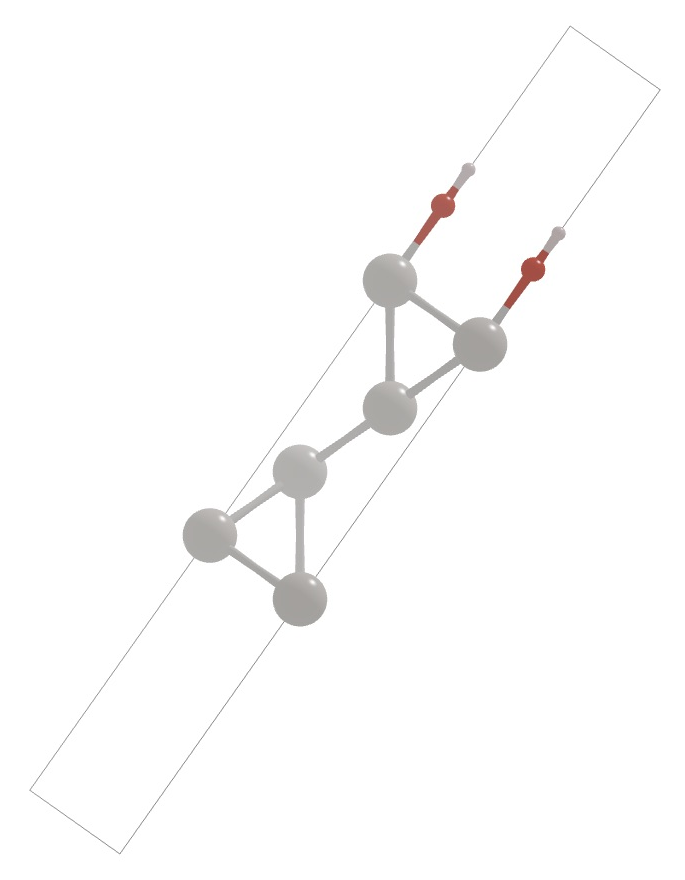
\includegraphics[width=\linewidth]{publication-assets/crop-c201c0495d5d847c2fd3.png}
\end{minipage}\hfill
\begin{minipage}[t]{40mm}
\vspace{0pt}
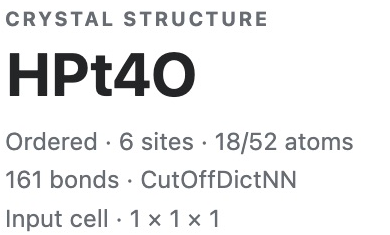
\includegraphics[width=\linewidth]{publication-assets/crop-5caa5064e4762ffc4974.png}
\end{minipage}
\caption{Side view after applying adsorption placement and wrapping with a $1\times1\times1$ unit supercell. The $\mathrm{Pt_4OH}$ model has 6 independent sites. The two displayed O--H groups are periodic images of one fragment. This is the initial placed geometry.}
\label{fig:pt111-oh-side}
\end{figure}


The reference is $\mathrm{Pt_4OH}$ with 6 sites. O is $2.00\,\text{\AA}$ above the top plane and H is $2.96\,\text{\AA}$ above it; the O--H length remains $0.96\,\text{\AA}$. Use \file{Pt111-OH-outward.cif} to compare cell and positions; the explicit single bond is retained in the input MOL file. Setting orientation atom to 0 preserves the fragment's original orientation, so equal anchor heights need not produce equal orientations.

The supplied \file{Pt111-OH-Online-050.json} contains the wrapped six-site model with the same periodic geometry, ready for viewing and further editing. Adsorption energy requires subsequent calculations.

\subsection{Compare adsorption configurations in a batch}

\ui{Adsorption Locator} enumerates sites, heights, and rotations and retains candidates by score. Import a fresh \file{Pt111-normal-c.json}, activate the clean four-site host, and select the same O--H molecule. Enter \literalinput{ontop bridge hollow} under \ui{Site types} and \literalinput{1.8 2.1 2.4} under \ui{Candidate heights (Å)} to compare $1.8$, $2.1$, and $2.4\,\text{\AA}$. Set anchor atom to 1 and orientation atom to 0. Use rotation step $30^\circ$, minimum contact distance $0.6\,\text{\AA}$, at most 200 retained candidates, and seed 0. Keep the default geometric contact score.

These parameters produce 144 candidates. Each retains the O--H bond length and places its anchor at the specified height along the surface normal. \file{Pt111-OH-candidate-1.json} is the highest-ranked geometric result: hollow candidate 2, height $2.4\,\text{\AA}$, and rotation $60^\circ$. Compare it with the earlier ontop model, then inspect the anchors and rotations of other candidates.

These values illustrate the search space. For a larger molecule, begin with fewer height and rotation combinations, confirm the anchor settings, then broaden the search. Select a candidate, \ui{Preview} and compare it with others, then \ui{Apply} the required configuration. Retain clearly named separate models for configurations that will be relaxed independently.

The default geometric contact score measures geometric suitability. The optional UFF van der Waals interaction energy estimates interactions in a rigid model. Both screen starting structures; neither replaces an adsorption energy after relaxation. Record the configuration's origin and the subsequent calculation method when reporting results.

\section{Treat surface boundaries}

\subsection{Passivate an unsaturated surface}

\ui{Passivate Surface} adds atoms to undercoordinated surface sites. Settings include passivating element, bond length, upper/lower surface selection, and detection depth. Defaults are H, $1.1\,\text{\AA}$, both surfaces, and $1.5\,\text{\AA}$. Choose bond lengths and coordination appropriate to the desired chemistry. A target coordination of 0 lets the tool infer it; specify it explicitly when the surface chemistry is known.

\subsection{Add a solvent layer}

\ui{Add Solvent Layer} packs solvent molecules from the project above the surface. Prepare and check one solvent molecule first, then set molecule count, layer thickness, surface gap, and remaining vacuum. A readily inspected exercise might use 20 molecules, thickness $10\,\text{\AA}$, gap $2\,\text{\AA}$, and remaining vacuum $5\,\text{\AA}$. Contact tolerance and seed affect the packing. Inspect its extent from the side and local packing from above.

\section{Build a heterojunction}\label{sec:heterojunction}
\index{Layer matching}
\index{Heterojunctions}

\subsection{Understand the shared cell}

A heterojunction brings two different materials into contact. For a layered interface, prepare each material as a slab and stack them along the normal. Their original lattices generally differ. A periodic model needs a common in-plane cell and a decision about acceptable deformation. That cell defines both interface periodicity and the atom count of a calculation.

\ui{Stack Heterostructure} builds such vertically stacked interfaces. It compares in-plane supercells and rotations, then assembles the parts at the chosen separation. Graphene/h-BN is a small, easily inspected example. For thin-film interfaces from bulk materials, first use \ui{Build Slab} for each desired face and check layers, terminations, and composition before matching. Equal material names do not imply equal surface orientations: choose the planes before assembling the interface.

In-plane strain measures how much the original lattices change to share a period. Interlayer spacing is the initial separation, and in-plane translation changes local registry. Each plays a different role. After constructing the geometry, compare separations and stacking arrangements using consistent calculations. Interfacial charge transfer and band alignment are properties of the subsequent electronic structure calculation.

\subsection{Insert a structure by translation}

\ui{Insert Structure} places another project structure into the active model using a Cartesian translation and minimum interatomic distance. Use it when the relative positions are already known. After insertion, check the cell, composition, and close contacts across boundaries.

\subsection{Find an in-plane lattice match}

\ui{Stack Heterostructure} searches in-plane lattice matches. Choose the top structure and specify layer spacing, total vacuum, maximum in-plane strain, repetition range, and rotation range. The default spacing of $3.35\,\text{\AA}$ is only an initial value, not a universal spacing for all materials. Maximum strain 0.03 means 3\% and is dimensionless. Candidates can be sorted by strain, area, or atom count.

First assess whether the strain is appropriate, then whether cell area and atom count are affordable. The lowest-strain candidate need not be the smallest. After selecting a match, check in-plane orientation, layer separation, and vacuum, and save different stackings separately.

\subsection{Exercise: compare insertion with layer matching}

The supplied \file{graphene-layer.json} contains two C sites, an in-plane lattice constant of $2.46\,\text{\AA}$, and box height $15\,\text{\AA}$. It is periodic in-plane and nonperiodic along the normal. Import it twice and name the structures \file{bottom} and \file{top} to practice on a same-material bilayer.

For direct insertion, activate the bottom layer, open \ui{Insert Structure}, and choose the other project structure as the top layer. Enter 0, 0, 3.35 in the three \ui{Cartesian translation (Å)} fields and retain minimum distance $0.5\,\text{\AA}$. The result should contain 4 sites, with layers $3.35\,\text{\AA}$ apart and the original box height of $15\,\text{\AA}$. \file{graphene-inserted.json} preserves this result.

Start again from the original bottom layer and open \ui{Stack Heterostructure}, using \file{top}. Set spacing to $3.35\,\text{\AA}$, total vacuum to $15\,\text{\AA}$, maximum strain to 0.03, maximum in-plane repetition to 2, and maximum rotation search angle to $0^\circ$. Sort by area.

Set \ui{Interface candidate index} to 1, preview and apply, then inspect the candidate table. The reference lists 10 candidates. Candidate 1 has zero strain and an estimated 4 sites. Applying it gives a bilayer with box height $18.35\,\text{\AA}$ and layer spacing $3.35\,\text{\AA}$, saved as \file{graphene-stacked.json}. Direct insertion preserves the original box, whereas matching rebuilds the normal dimension from the slab and total vacuum.

The list may include combinations above the requested strain limit; being listed does not mean that they can be applied. Candidates 2 and 3 here have approximately 52.49\% strain and should be excluded. Candidates 4, 5, and 6 have nearly zero strain but require 8 sites. Check constraints before choosing a suitable area or size rather than relying on the atomic picture alone.

\subsection{Example: match graphene and h-\headinglatin{BN}}

Different materials usually have slightly different in-plane dimensions. Here graphene is stacked with hexagonal boron nitride (h-BN) to inspect the matching strain. \file{hBN-layer.json} is an ideal monolayer with one B and one N site and in-plane lattice constant $2.50\,\text{\AA}$, compared with graphene's $2.46\,\text{\AA}$. Both inputs have normal box height $15\,\text{\AA}$.

\begin{steps}
  \item Import \file{graphene-layer.json} and \file{hBN-layer.json} into one project. Activate the newly imported \file{graphene-layer}, open \ui{Stack Heterostructure}, and choose \file{hBN-layer} under \ui{Top-layer structure}.
  \item Set spacing to $3.35\,\text{\AA}$, total vacuum to $15\,\text{\AA}$, and maximum in-plane strain to 0.03.
  \item Set maximum in-plane repetition to 1 and maximum rotation search angle to $0^\circ$. Sort by strain. This narrow initial search makes the lattice matching easy to understand.
  \item Set \ui{Interface candidate index} to 1, preview and apply, then inspect the spacing from the side. The result table has one candidate: in-plane strain 0.016, or 1.6\%, with an estimated 4 sites.
\end{steps}

The candidate table is for inspection and has no button for applying a different configuration within the table. To compare another candidate, undo to the original bottom layer or import it again, reopen the command, and enter the required index. Do not keep adding layers to an assembled bilayer.

The result, \file{graphene-hBN-stacked.json}, contains $\mathrm{C_2BN}$. The h-BN in-plane lattice is matched to graphene; layer spacing is $3.35\,\text{\AA}$ and normal box height $18.35\,\text{\AA}$. Unlike the same-material bilayer, this pair needs finite in-plane deformation to share a cell. Broaden the repetition and rotation ranges later to compare larger matches, saving each configuration intended for calculation. The entered spacing is a modeling starting value; relaxation determines the resulting distance.

\section{Build a twisted bilayer}\label{sec:twisted-structures}
\index{Twisted bilayers}
\index{Moire superlattices@Moiré superlattices}

\subsection{From a relative rotation to a common period}

Place two graphene monolayers on top of each other and rotate one about the surface normal. Their local registry then varies across the plane: in some regions atoms nearly coincide vertically, while elsewhere an atom in one layer lies near the center of a hexagon in the other. Viewed over a larger area, these local arrangements form a repeating moiré pattern.

A periodic calculation also needs a common cell. Simply rotating the upper layer within its original small cell generally leaves the two layers incompatible across the boundaries. \ui{Twist Moiré Superlattice} selects an integer supercell for each layer so that both fit a shared in-plane period. The target angle guides the search, while a particular set of integer relations defines the resulting model.

The first example is a graphene bilayer twisted by approximately $21.7868^\circ$. Its relatively short common period gives only 28 carbon sites, making the layers and cell easy to inspect. Complete this example before trying smaller angles to understand how angle, period, and model size are related.

\subsection{Prepare the two layers}

The tool uses hexagonal in-plane primitive cells: the two in-plane vectors have equal lengths and enclose $60^\circ$ or $120^\circ$. Each input graphene monolayer here contains two C sites, has an in-plane lattice constant of $2.46\,\text{\AA}$, and a box height of $15\,\text{\AA}$. It is periodic in both in-plane directions and nonperiodic along the normal.

The supplied \file{twist-graphene-bottom.json} and \file{twist-graphene-top.json} come from the same monolayer input, with the same geometry as \file{graphene-layer.json} used earlier. Separate filenames identify their roles in the project; they do not mean that a relative rotation has already been applied.

\begin{steps}
  \item Import both JSON files into one project and name the structures \file{twist-bottom} and \file{twist-top}.
  \item Open the bottom layer's 3D document and check that it has two model sites. More than two atoms may be displayed to show periodic connections.
  \item Inspect the lattice: both in-plane lengths should be $2.46\,\text{\AA}$ and their angle approximately $120^\circ$. Check that the top layer has the same lattice and composition.
  \item Activate \file{twist-bottom}. On \ui{Crystal Modeling}, open \ui{Interface Modeling} in \ui{Surfaces \& Interfaces}, then choose \ui{Twist Moiré Superlattice}.
  \item Select \file{twist-top} under \ui{Top-layer structure}. Choose an existing project structure rather than entering a disk path.
\end{steps}

Begin with these two original monolayers. Keep any bilayer created by insertion or stacking separately; it is no longer a single input layer for this exercise.

\subsection{Enter a small-model parameter set}

\begin{table}[htbp]
\centering
\caption{Parameters for the 28-site twisted graphene bilayer.}
\begin{tabularx}{\linewidth}{lX}
\toprule
Parameter & Input and meaning\\
\midrule
Top-layer structure & Select \file{twist-top}.\\
Angle (degrees) & Enter \literalinput{21.786789} as the target relative angle.\\
Interlayer gap (Å) & Enter 3.35 for the initial separation between layers.\\
Total vacuum thickness (Å) & Enter 15 for the total empty height outside the slab.\\
Maximum in-plane strain & Enter 0.03, or 3\%.\\
Maximum atom count & Enter 200 as the upper limit on total model sites.\\
Maximum coincidence index & Enter 6 to bound the integer matching search.\\
\bottomrule
\end{tabularx}
\end{table}

\ui{Angle (degrees)} is a numeric field; enter the value without a degree symbol. \ui{Interlayer gap (Å)} and \ui{Total vacuum thickness (Å)} are also numerical lengths. Maximum strain is a fraction: 0.03 means 3\%; entering 3 would specify a different requirement.

The atom limit does not request exactly 200 atoms. Likewise, \ui{Maximum coincidence index} limits the search over integer coincidence relations; it does not simply repeat a direction six times. Within the search bounds, the tool considers angle error, strain, and model size and selects an integer match. These limits therefore differ from the three repeat factors in \ui{Build Supercell}.

This command selects one match internally. Unlike \ui{Stack Heterostructure}, it has no candidate ranking or candidate-index field. Check the actual size and relative orientation after construction. To compare other matches, retain the original layers and generate and save separate results for each parameter set.

\begin{steps}
  \item Enter the table's values and click \ui{Preview}. The two-site monolayer should become a larger periodic structure containing two layers.
  \item Look nearly along the surface normal and check that the hexagons in the two layers are rotated relative to each other. Inspect the side view to confirm that there are still only two layers, with no unintended atoms between them.
  \item Check for 28 model sites. The expanded in-plane cell may display more atoms because of periodic images.
  \item Apply, name the result \file{graphene-twist-21p786789}, and save the project. Retain both monolayers so later comparisons can start from the same inputs.
\end{steps}

\begin{figure}[!htb]
\centering
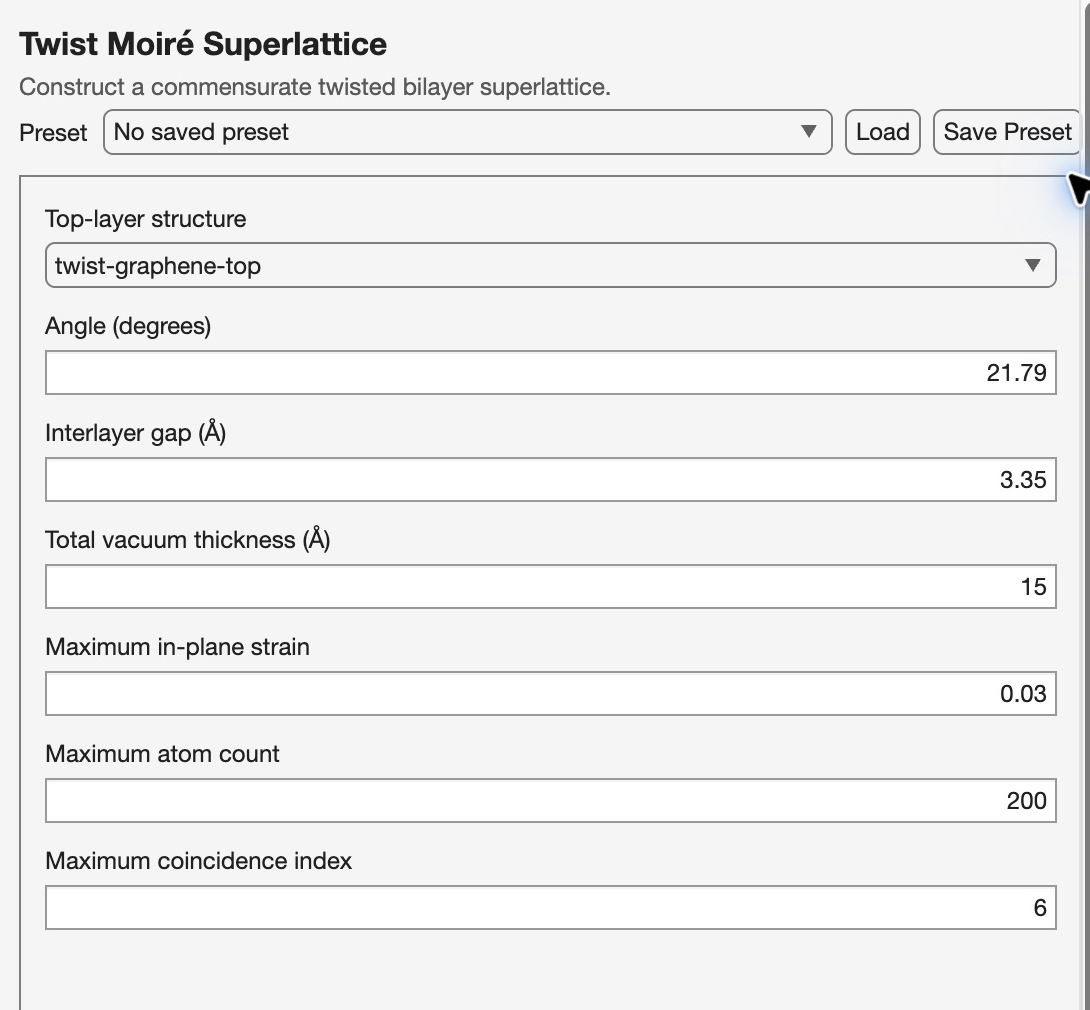
\includegraphics[width=107mm]{publication-assets/crop-7c221ceb9a35fdad53a3.png}
\par\vspace{2mm}

\includegraphics[width=107mm]{publication-assets/crop-faecdf5879e359505e34.png}
\caption{Twist parameters and preview. The entered target is 21.786789 degrees; after the field loses focus, it displays 21.79 at the available precision. The top layer retains its imported name, \file{twist-graphene-top}, corresponding to \file{twist-top} in the instructions. The preview contains 28 sites.}
\label{fig:online-twist-parameters}
\end{figure}

\begin{figure}[!htb]
\centering
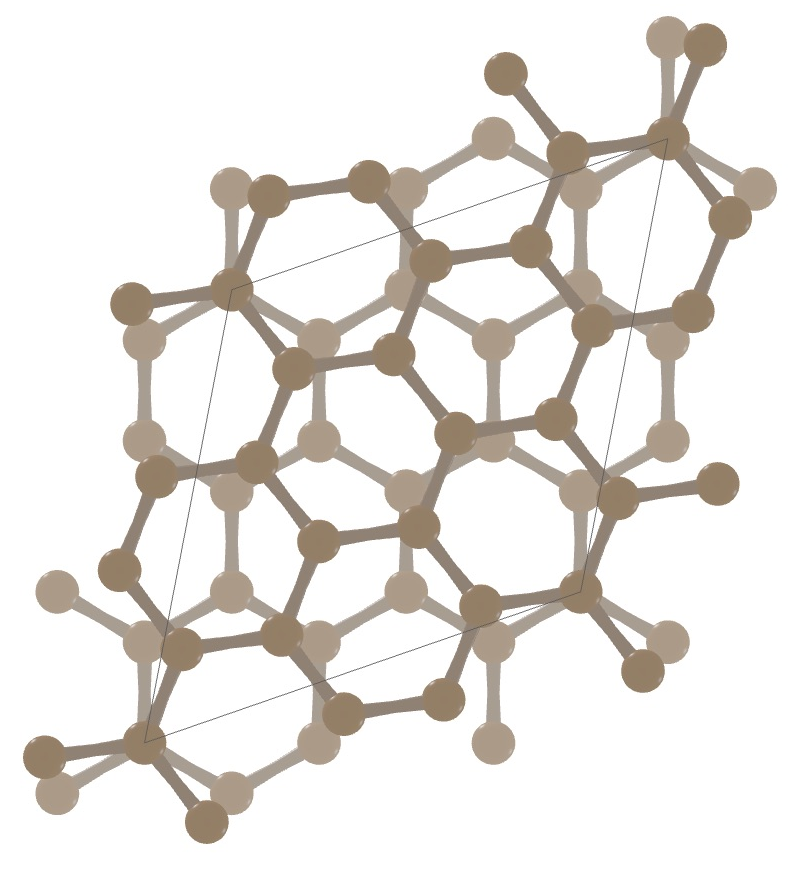
\includegraphics[width=93mm]{publication-assets/crop-89eb072a4598add87b05.png}
\caption{View along the normal of the twisted graphene bilayer. The hexagons are rotated relative to one another. The 28 model sites appear as 68 displayed atoms at the current periodic display range.}
\label{fig:online-twist-top}
\end{figure}

\subsection{Interpret the generated cell}

The supplied \file{graphene-twist-21p786789.json} is the reference structure generated with these parameters; a CIF with the same base name is provided for geometry exchange. The model contains 28 C sites, 14 in each layer. Each layer's in-plane area is seven times that of the original two-site monolayer.

Both in-plane vectors are approximately $6.508548\,\text{\AA}$ long, giving an area of approximately $36.6859\,\text{\AA}^2$. The new cell angle is $60^\circ$, whereas the input primitive cell uses $120^\circ$. These are different lattice-basis representations; the angle change alone does not establish that the crystal has been distorted. Check lengths, area, site count, and periodic connectivity together.

For these graphene inputs, the period length can also be checked as $\sqrt{7}\times2.46\,\text{\AA}$, or approximately $0.651\,\mathrm{nm}$. This is the common cell's in-plane repeat length, not the interlayer separation or a C--C bond length. Each layer retains a shortest nearest-neighbor distance of approximately $1.420282\,\text{\AA}$, matching the input monolayer.

The side view shows a layer separation of $3.35\,\text{\AA}$ and a normal cell height of $18.35\,\text{\AA}$. Each layer is planar here, so the cell height is the layer separation plus the total vacuum. Total vacuum of $15\,\text{\AA}$ means all empty height outside the slab, not $15\,\text{\AA}$ on each side.

\begin{figure}[!htb]
\centering
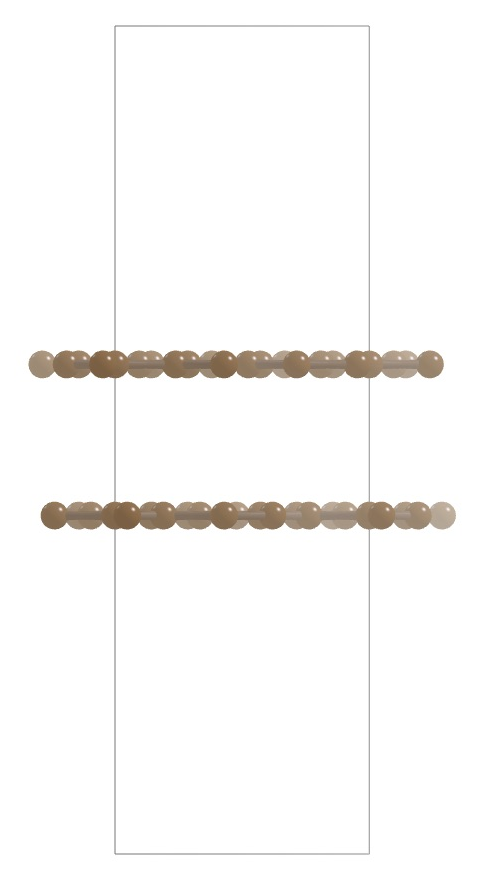
\includegraphics[width=67mm]{publication-assets/crop-a8d161a93e2745b16ef3.png}
\caption{Side view of the same model. The two atomic planes and the cell boundaries distinguish the interlayer gap from the external vacuum.}
\label{fig:online-twist-side}
\end{figure}

The reference model's achieved angle is $21.786789298^\circ$, approximately $2.98\times10^{-7}$ degrees from the target, with zero in-plane strain. The relative angle can also be obtained from nearest-neighbor bond directions in the two layers.

Exact matching information is stored in the \file{moire} section under \file{properties} in the native JSON. Open the JSON in a text editor and search for \file{achieved_angle_degrees}. The fields \file{target_angle_degrees}, \file{angle_error_degrees}, and \file{in_plane_strain} record the target, angle error, and in-plane strain. For your own structures, choose \ui{Export file → Structure file}, then export JSON. Do not choose \ui{Scene JSON}: it records the viewing scene rather than the structural matching information.

\subsection{Why the achieved angle may differ from the target}

Target angles range from $0^\circ$ to $60^\circ$. Using hexagonal in-plane symmetry, the tool represents achieved matching angles between $0^\circ$ and $30^\circ$. Apply that convention when comparing larger targets. The example stays within the smaller range so that target and achieved values can be compared directly.

A common period requires particular integer relations. An arbitrary decimal angle need not have a reasonably sized periodic cell that matches it exactly. Changing the target to $22^\circ$ while retaining the other settings still gives 28 sites and an achieved angle of approximately $21.786789298^\circ$, now with an error of approximately $0.213211^\circ$.

The two constructions have the same final geometry but different target inputs. The supplied \file{graphene-twist-target22.json} preserves the second result for comparison. Report the achieved angle rather than using only the target entered in the parameter dialog.

\begin{table}[htbp]
\centering
\caption{Effects of target angle and size limits for these inputs.}
\begin{tabularx}{\linewidth}{lX}
\toprule
Input change & Actual result\\
\midrule
Target $21.786789^\circ$, limit 200 & 28 sites; achieved angle approximately $21.786789298^\circ$.\\
Target $22^\circ$, limit 200 & The same 28-site geometry and achieved angle; error approximately $0.213211^\circ$.\\
Target $21.786789^\circ$, limit 24 & A four-site match close to $0^\circ$, missing the original target.\\
\bottomrule
\end{tabularx}
\end{table}

The third case shows why successful construction and an acceptable angle match are separate checks. Once the 28-site match is excluded by the limit of 24, the tool selects from the remaining search space. If the resulting size differs markedly from your expectation, check the parameters and achieved angle together before increasing the search bounds.

Smaller twist angles generally require longer common periods and more atoms. To compare angles, first hold layer spacing and strain requirements fixed, then gradually increase the allowed size and maximum coincidence index. This reveals whether the broader search improves the angle match or merely produces a larger structure. The approximately $21.8^\circ$ example uses small integers and is a useful starting point for learning the procedure and checking periodicity.

\subsection{Choose an assembly tool for your purpose}

The \ui{Interface Modeling} menu groups several assembly methods. Decide which geometric relationships are already known and which ones the tool should find.

\begin{table}[htbp]
\centering
\caption{Choosing insertion, lattice matching, or twist construction.}
\begin{tabularx}{\linewidth}{lX}
\toprule
Tool & Suitable starting situation\\
\midrule
Insert Structure & The two parts already have defined positions; specify a translation and retain the current host cell.\\
Stack Heterostructure & Compare common in-plane cells using allowed strain, repetition, and rotation ranges.\\
Twist Moiré Superlattice & Start from hexagonal monolayers and a target angle, then find a common period from integer lattice relations.\\
\bottomrule
\end{tabularx}
\end{table}

In the \ui{Stack Heterostructure} candidate table, area, strain, atom count, and rotation each answer a different question. Area and atom count indicate calculation size; strain measures the change needed to match the original lattices; rotation defines their relative orientation. A low-strain candidate can be large, while the smallest-area candidate may require substantial deformation. Compare these quantities before inspecting the atomic arrangement.

The twist command instead uses hexagonal integer relations to select a common period, then assembles the layers. It does not ask for a candidate index in the same dialog. To compare targets of $21.786789^\circ$ and $22^\circ$, build each result from the two original monolayers and record them separately. Do not apply the command again to an already assembled bilayer.

Rotating the camera only changes the viewpoint; rotating selected atoms changes their positions. Neither replaces periodic matching of the shared cell. Alongside layer orientation, display the cell boundaries and inspect repetitions along both in-plane directions to ensure that the local pattern and full periodic cell describe the same model.

These tools assemble layered interfaces along the normal. An in-plane lateral heterojunction requires separate preparation of the junction's atomic arrangement and boundaries.

\subsection{Build a twisted graphene/h-\headinglatin{BN} heterostructure}

Twisting also applies to layers of different materials. The earlier zero-angle graphene/h-BN match illustrates how different in-plane lattice constants are accommodated. A relative rotation can be introduced as well. Here graphene is the bottom layer with lattice constant $2.46\,\text{\AA}$, and h-BN is the top layer with $2.50\,\text{\AA}$.

\begin{steps}
  \item Import \file{twist-graphene-bottom.json} and \file{hBN-layer.json} afresh, naming them \file{graphene-bottom} and \file{hBN-top}. Do not use the previously twisted bilayer as the bottom layer.
  \item Activate the new graphene monolayer. In \ui{Twist Moiré Superlattice}, choose \file{hBN-top} under \ui{Top-layer structure}.
  \item Retain the table's target angle, layer separation, total vacuum, 200-site limit, and maximum coincidence index of 6. Keep maximum in-plane strain at 0.03.
  \item Preview and check for $\mathrm{C_{14}B_7N_7}$ with 28 total sites. Each layer has 14 sites, but their elements differ.
  \item Apply and save as \file{graphene-hBN-twist-21p786789}, then compare with the zero-angle \file{graphene-hBN-stacked.json}.
\end{steps}

The achieved angle is again approximately $21.786789298^\circ$. The principal in-plane strain is 0.016, or 1.6\%. The h-BN dimensions are matched to the common graphene lattice, while separation remains $3.35\,\text{\AA}$ and normal cell height remains $18.35\,\text{\AA}$. Strain changes dimensions; twist changes relative orientation. They describe different modifications.

Both construction commands produce geometric models. To study interfacial charge transfer, band alignment, or junction properties, build the appropriate calculations on the saved structures and distinguish the input layer separation from the distance obtained after calculation.

\subsection{Save twisted models}

A project retains the input layers, generated structures, and later workflows. JSON and CIF are supplied for structure exchange. JSON preserves in-plane/normal periodicity flags, layer indices, and twist-matching metadata. CIF is used to exchange the cell and atomic positions. These CIF files are imported as periodic in all three directions, and moiré metadata must be retained separately. Prefer JSON for further 2D modeling comparisons here. When using CIF in another calculation, check normal boundary conditions and vacuum for the target method.

\begin{steps}
  \item Give each result a name identifying the material, achieved angle, and main change, such as ``graphene bilayer, achieved angle 21.7868 degrees,'' rather than a generic \file{result}.
  \item Record the input lattices, target and achieved angles, strain, layer separation, total vacuum, site count, and in-plane period. Use a separate comparison-table column for each quantity.
  \item Reopen the saved project and check both layers' composition and the cell. Keep the parameter record with an exported structure so its geometry can be interpreted in other software.
  \item To regenerate the examples, start MATLAB\regmark{} with \file{-nojvm}, configure the toolbox path, and run \file{twist_examples.m} from the supplied examples directory. To check saved files only, run \file{verify_twist_examples.m}.
\end{steps}

The supplied structures are starting models for relaxation and electronic structure calculations. When comparing twist effects, use consistent functionals, pseudopotentials, cutoffs, and suitable sampling, and save those settings with the structures.


\section{Prepare an initial \headinglatin{NEB} path}

\ui{Interpolate NEB Path} uses initial and final project structures. They must have identical atom counts, element order, and lattices so that atoms correspond one to one. By default, it generates 5 intermediate images and uses IDPP to improve interpolation distances. Inspect every image for motion and close contacts. These structures initialize a later path calculation; the reaction barrier requires energy calculations.

\subsubsection{How intermediate images are distributed}

Requesting $M$ intermediate images produces $M+2$ structures including both endpoints, indexed by $j=0,\ldots,M+1$. For a nonperiodic model, or endpoints represented by continuous periodic images, linear interpolation gives
\begin{equation}
  \alpha_j=\frac{j}{M+1},\qquad
  \mathbf r_i^{(j)}=(1-\alpha_j)\mathbf r_i^{(0)}
     +\alpha_j\mathbf r_i^{(M+1)}.
  \label{eq:neb-image-interpolation}
\end{equation}
Index $i$ identifies the same atom at both endpoints; $\alpha_j$ is dimensionless and positions are in \AA. For periodic structures, endpoint displacements must respect the applicable periodic boundaries. Coordinates of different images of one atom must not be interpreted as an unnecessarily long migration distance.

IDPP further brings pair distances in each image toward interpolated targets:
\begin{equation}
\begin{aligned}
  d_{ik}^{*,(j)}&=(1-\alpha_j)d_{ik}^{(0)}
                      +\alpha_j d_{ik}^{(M+1)},\\
  E_{\mathrm{IDPP}}^{(j)}&=
    \sum_{i<k}\frac{\bigl(d_{ik}^{(j)}-d_{ik}^{*,(j)}\bigr)^2}
                         {\bigl(d_{ik}^{(j)}\bigr)^4}.
\end{aligned}
\label{eq:idpp-pair-objective}
\end{equation}
Here $i,k$ are atom indices and $j$ is an image index. The current pair distance is $d_{ik}^{(j)}$ and its target is $d_{ik}^{*,(j)}$. The denominator strongly penalizes short separations, helping IDPP resolve collisions in a linear path. This expression describes one image's pair objective; path optimization also couples neighboring images.

$E_{\mathrm{IDPP}}$ is an auxiliary geometric objective, not a reaction barrier. A barrier requires subsequent energy calculations. The dialog's IDPP \ui{Force tolerance} applies to this auxiliary optimization and is separate from electronic-structure force thresholds. For $M=5$, the parameters are $0,1/6,2/6,\ldots,1$, corresponding to example structures 00 through 06.


\subsection{Exercise: inspect five intermediate images}
\index{NEB paths}

The supplied \file{neb-exchange/initial.json} and \file{final.json} provide a geometric example with clear atom correspondence. Two differently labeled H atoms exchange positions in a nonperiodic cubic box of side $10\,\text{\AA}$. The initial positions are $(2,5,5)$ and $(8,5,5)\,\text{\AA}$; the final structure swaps them. This tests how interpolation avoids overlap, rather than modeling a hydrogen molecule reaction.

\begin{steps}
  \item Import both endpoint files, naming them \file{initial} and \file{final}. Check atom order and labels, then activate the initial structure.
  \item On \ui{Crystal Modeling}, open \ui{Interface Modeling} in \ui{Surfaces \& Interfaces}, then choose \ui{Interpolate NEB Path}. Select the project structure \literalinput{final} under \ui{Endpoint structure}.
  \item Set \ui{Intermediate image count} to 5, retain \ui{Maximum optimization steps} of 200 and \ui{Force tolerance} of 0.1 for IDPP. Preview and apply, then open \literalinput{NEB image 00} through \literalinput{NEB image 06} from the Project Browser. The seven structures include both endpoints and five intermediate images.
  \item Inspect the labels and distance in sequence. Endpoints should retain their original coordinates, while intermediate images avoid the position where the atoms would overlap. Saving the project retains both input endpoints and all seven results. Export individual structures when needed.
\end{steps}

Straight-line interpolation makes the atoms coincide in the middle image. The reference IDPP path reaches its threshold in 82 iterations. The minimum pair separation along the path is approximately $3.5755\,\text{\AA}$, and the middle image has approximately $3.7380\,\text{\AA}$. Files \file{image-00.json} through \file{image-06.json} preserve every image. IDPP objective values and numerical forces assess the initial path; they are not electronic structure energies or atomic forces.

Figure~\ref{fig:neb-idpp} compares these coordinates with linear interpolation. Lines on the left connect the generated images; the right panel gives their pair distances. Following the image numbers checks both fixed endpoints and improved intermediate contacts.

\begin{figure}[H]
\centering
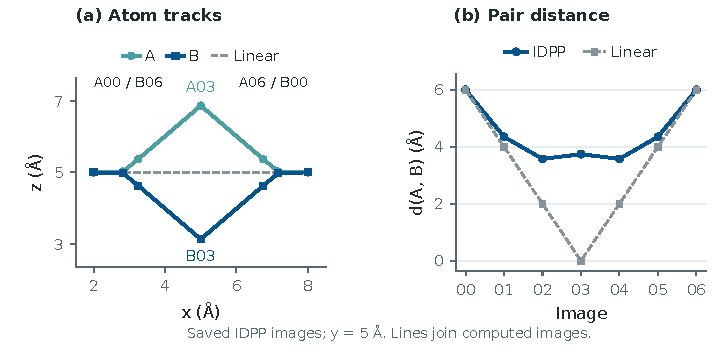
\includegraphics[width=\linewidth]{publication-assets/vector-79e6f35b7afec0271551.pdf}
\caption{Reference IDPP path for two exchanging atoms. Left: $x$--$z$ trajectories at fixed $y=5\,\text{\AA}$; labels such as A00/B06 identify endpoint correspondence. Right: pair separations for images 00--06. Gray dashed lines show linear interpolation; 03 is the middle image.}
\label{fig:neb-idpp}
\end{figure}

\section{Example: build low-dimensional models}\label{sec:nanostructure-examples}
\index{Nanoribbons}\index{Nanotubes}\index{Nanowires}

Cutting a sheet into a ribbon or rolling it into a tube changes its boundaries and periodicity. A ribbon has edges across its width and repeats only along its length. A nanotube repeats along its axis, with vacuum in the other directions. A wire cut from a bulk crystal likewise has one periodic direction, whereas a finite cluster is nonperiodic in all three.

This section first builds a 24-site graphene ribbon and a 32-site nanotube from a small primitive cell, then uses face-centered cubic copper to build a wire, finite cluster, and spherical void. Native JSON and CIF files accompany every result for comparison as you work.

\subsection{Prepare a 60-degree graphene primitive cell}

The supplied \file{nano-graphene-60.json} has two C sites, equal in-plane vector lengths of $2.46\,\text{\AA}$, an angle of $60^\circ$, and normal box height $15\,\text{\AA}$. It is periodic in-plane and nonperiodic along the normal. It represents the same graphene sheet as \file{graphene-layer.json}, using a different lattice basis.

Starting from the earlier $120^\circ$ cell, retain $\mathbf a$ and replace the second vector by $\mathbf a+\mathbf b$. The new vector still has length $2.46\,\text{\AA}$, but forms $60^\circ$ with $\mathbf a$. This integer basis change has determinant 1, so the model still has two independent sites. Both ribbon and tube examples use this $60^\circ$ input.

\begin{steps}
  \item Import \file{nano-graphene-60.json}, name it \file{nano-graphene}, and open its 3D document. Check for two independent sites, equal in-plane lengths, and $60^\circ$.
  \item To perform the basis change yourself, separately import and activate \file{graphene-layer.json}. Open \ui{Build Supercell} under \ui{Crystal Modeling}\,$\rightarrow$\,\ui{Supercell \& Lattice}.
  \item Enter \literalinput{1 0 0; 1 1 0; 0 0 1} under \ui{Supercell scaling}. This is a three-row integer matrix, with semicolons separating rows; it differs from editing individual cells in the lattice editor.
  \item Preview and check that the site count remains 2, volume is unchanged, and the in-plane angle becomes $60^\circ$. Apply and save under a basis-specific name without overwriting the $120^\circ$ monolayer.
  \item Retain separate inputs for the ribbon and nanotube. Start each construction from a monolayer; rolling an already cut ribbon would be a different procedure.
\end{steps}

The two cell boundaries look different, but describe the same periodic material. Check the input and basis before comparing site counts and dimensions. Widths or chiral indices alone do not fully specify the construction.

\subsection{Cut an armchair graphene nanoribbon}

Ribbon width and axial length are entered as repeat-unit counts; vacuum is in \AA. \ui{Armchair} and \ui{Zigzag} describe edge arrangements, not camera directions. Here choose armchair, inspect the paired carbon arrangement along the edges, then check connectivity along the periodic length.

\begin{table}[htbp]
\centering\small
\caption{Parameters for the 24-site armchair ribbon.}
\begin{tabularx}{\linewidth}{lX}
\toprule
Field & Input\\
\midrule
Width repetitions & 3, a dimensionless integer.\\
Axial repetitions & 2, a dimensionless integer.\\
Edge type & \ui{Armchair}.\\
Vacuum (Å) & 5; the tool adds this much on each side in both nonperiodic directions.\\
Maximum atom count & 500, an upper bound rather than a requested final count.\\
\bottomrule
\end{tabularx}
\end{table}

\begin{steps}
  \item Activate the prepared \file{nano-graphene} monolayer. Open \ui{Cut Nanoribbon} from \ui{Nanostructures} on \ui{Crystal Modeling}.
  \item Enter the table's values. Width 3 is not $3\,\text{\AA}$, and axial count 2 is not $2\,\text{\AA}$.
  \item Click \ui{Preview} and show the cell boundary. Inspect both edges along the sheet normal, then check from the side that the model is still flat.
  \item Check for 24 independent C sites. Inspect the periodic connections along the ribbon; the network near the two cell ends is not two disconnected molecules.
  \item Apply, name the result \file{graphene-armchair-w3-l2}, and save. Compare with the supplied JSON of the same name and retain the original monolayer separately.
\end{steps}

The result is periodic along global $y$, with native flags \literalinput{false true false}. Cell lengths are approximately $16.15$, $8.521690$, and $10.00\,\text{\AA}$. The axial period is $8.521690\,\text{\AA}$. The atoms span $6.15\,\text{\AA}$ across the width, plus $5\,\text{\AA}$ vacuum on each side, giving $16.15\,\text{\AA}$. The flat sheet has no normal thickness, so its normal box length is $10\,\text{\AA}$.

For the 24 unpassivated C atoms, a neighbor cutoff of $1.65\,\text{\AA}$ gives 16 atoms with three neighbors and 8 edge atoms with two. The shortest periodic distance is approximately $1.420282\,\text{\AA}$. This cutoff checks this carbon model; it is not a universal bonding distance. For hydrogen-passivated edges, save the unpassivated structure first, add hydrogen according to the intended edge coordination, and check composition.

\subsection{Roll graphene into a small nanotube}

First identify which in-plane vector becomes the circumference. The geometry described in the help is
\begin{equation}
  \mathbf C_h=n\mathbf a_1+m\mathbf a_2,
  \qquad R=\frac{\|\mathbf C_h\|}{2\pi}.
  \label{eq:nanotube-circumference-radius}
\end{equation}
Here $\mathbf a_1,\mathbf a_2$ are the input in-plane vectors in \AA; $n,m$ are dimensionless chiral indices; $\mathbf C_h$ is the chiral vector; and $R$ is the initial radius. The circumference is the magnitude of that vector combination. Vectors of equal length enclosing $60^\circ$ give $\|\mathbf C_h\|=a\sqrt{n^2+nm+m^2}$. For another basis, use Eq.~\eqref{eq:nanotube-circumference-radius} directly. This section retains the prepared $60^\circ$ basis: the same $(n,m)$ in different bases need not select the same rolling direction.

\begin{figure}[htbp]
\centering
\begin{tikzpicture}[x=1mm,y=1mm,font=\sffamily\small,>=stealth]
  \node[text=brand] at (26,54) {Rolling direction};
  \foreach \j in {0,1,2,3} {
    \draw[teal!55] ({6+4*\j},{10+7*\j}) -- ({38+4*\j},{10+7*\j});
    \foreach \i in {0,1,2,3,4} {
      \fill[brand] ({6+8*\i+4*\j},{10+7*\j}) circle (.8);
    }
  }
  \foreach \i in {0,1,2,3,4}
    \draw[teal!55] ({6+8*\i},10) -- ({18+8*\i},31);
  \draw[->,brand,line width=.9pt] (6,10) -- (38,10)
    node[midway,below=3pt] {$\mathbf C_h=4\mathbf a_1$};
  \draw[->,muted] (6,10) -- (14,10) node[above] {$\mathbf a_1$};
  \draw[->,muted] (6,10) -- (10,17) node[left] {$\mathbf a_2$};
  \draw[->,teal,line width=.8pt] (57,24) -- (69,24);
  \node[text=muted,font=\sffamily\footnotesize] at (63,32) {Join};
  \node[text=brand] at (95,54) {Fixed circumference};
  \fill[paleblue] (81,10) rectangle (109,39);
  \draw[brand,line width=.8pt] (81,10) -- (81,39);
  \draw[brand,line width=.8pt] (109,10) -- (109,39);
  \draw[brand,fill=paleblue,line width=.8pt] (95,39) ellipse (14 and 5);
  \draw[brand,line width=.8pt] (81,10) arc[start angle=180,end angle=360,x radius=14mm,y radius=5mm];
  \draw[brand,densely dashed] (109,10) arc[start angle=0,end angle=180,x radius=14mm,y radius=5mm];
  \draw[->,muted] (95,39) -- (109,39) node[midway,above] {$R$};
  \draw[->,teal] (115,10) -- (115,43) node[above] {Axis};
  \node[align=center,font=\sffamily\footnotesize] at (95,-1) {$\|\mathbf C_h\|=2\pi R$};
\end{tikzpicture}
\caption{Chiral vector and tube radius (schematic). The left panel shows lattice translation points and the $(4,0)$ direction that rolls into one circumference. The right panel relates the resulting circumference to its radius.}
\label{fig:nanotube-chiral-geometry}
\end{figure}


The chiral indices $(n,m)$ specify the circumferential lattice direction; axial repetitions set the number of translational periods along the tube. The small-radius $(4,0)$ example makes rolling, the seam, and periodicity easy to inspect. A relaxed equilibrium radius requires geometry optimization.

\begin{steps}
  \item Open a fresh monolayer from \file{nano-graphene-60.json} and activate it. Do not use the ribbon just created.
  \item Choose \ui{Roll Nanotube} under \ui{Nanostructures}. Enter 4 and 0 in the two \ui{Chiral indices (n m)} fields.
  \item Set \ui{Axial repetitions} to 2, \ui{Vacuum (Å)} to 6, and \ui{Maximum atom count} to 500.
  \item Preview the circular cross-section along the axis, then inspect the tube from the side. Rotate the camera to examine the seam and check periodic connections at the axial ends.
  \item Check for 32 C sites. Apply and save as \file{graphene-tube-4-0-l2}, retaining both monolayer and nanotube.
\end{steps}

The example is periodic along global $z$, with flags \literalinput{false false true}. Its rolling radius is
\[
 R=\frac{4\times2.46}{2\pi}\,\text{\AA}\approx1.566085\,\text{\AA}.
\]
Both transverse cell lengths are approximately $15.132169\,\text{\AA}$, the diameter plus $6\,\text{\AA}$ vacuum on each side. Axial length is approximately $8.521690\,\text{\AA}$. This transverse vacuum differs from total vacuum in the twisted-bilayer dialog; use each command's definition when checking box dimensions.

A periodic neighbor check on the saved coordinates finds three neighbors within $1.65\,\text{\AA}$ for every site, with a shortest distance of approximately $1.393202\,\text{\AA}$. Rolling a flat sheet onto a small circumference changes straight-line pair distances. Do not require every rolled C--C distance to remain exactly $1.420282\,\text{\AA}$. Check radius, seam, neighbors, and periodicity together, then relax the geometry separately.

\subsection{Inspect the tube end and side}

Import \file{graphene-tube-4-0-l2.json} directly to practice viewing before comparing other chiral indices. Initially retain \ui{Input cell} and \ui{1 × 1 × 1} so that the view represents one saved model period.

\begin{steps}
  \item Select the JSON through \ui{Home → Structure → Import structure from file...}. In Online, upload and then import it. Open the document and check for C and 32 sites.
  \item Click \ui{c} in the viewer toolbar, whose tooltip is \ui{View along c axis}. The tube axis is parallel to $c$, so this looks through its mouth. Inspect the carbon ring and central hollow region.
  \item Click \ui{a} or \ui{b} for a side view. Keep the same zoom and inspect the axial extent and curved hexagonal network. If spheres obscure bonds, reduce \ui{Atom scale} under \ui{Viewer settings → Style}.
  \item Show \ui{Unit cell} under \ui{Visibility} and compare the tube with its transverse vacuum box. Hide \ui{Boundary image atoms} to inspect one period's atoms, then show them again to check end connections.
  \item Under \ui{Scientific scene → Repeat cell}, change only \ui{c} to 2 and inspect the axial join. Use \ui{Reset to 1 × 1 × 1} afterward, then \ui{Reset camera} for an overall view.
  \item Export end and side views, recording that they show the same 32-site structure, with $(4,0)$ chirality, two axial repeats, and the original JSON filename.
\end{steps}

The hole in the axial view confirms a tubular arrangement. The side and repeated views help establish its axial periodicity. Display repetition does not create a larger calculation supercell, and extra boundary spheres are scene images; obtain the independent site count from the structure. Together, these views communicate diameter, length, and periodicity more clearly than one perspective view.

\begin{figure}[!htb]
\centering
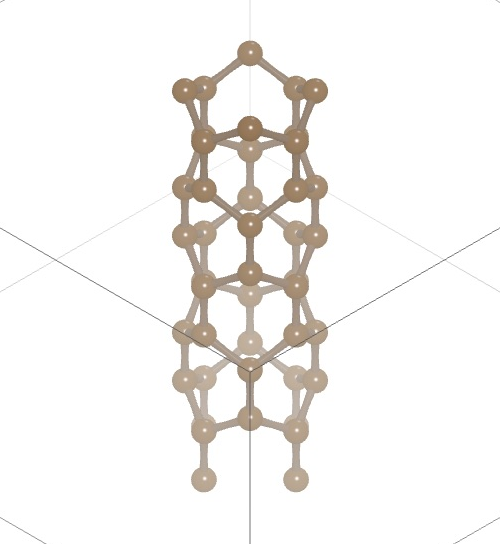
\includegraphics[width=.47\linewidth]{publication-assets/revision-nanotube-perspective.png}\hfill
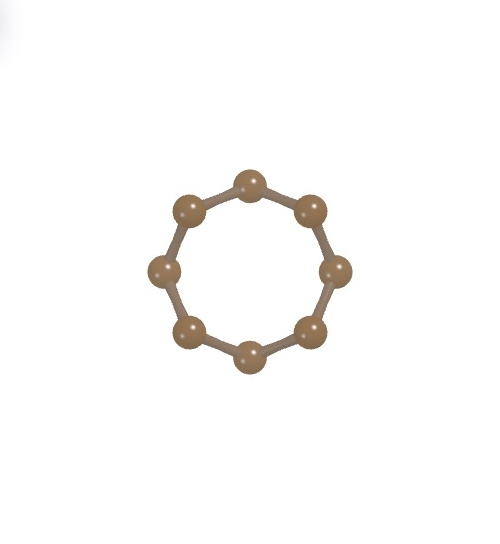
\includegraphics[width=.47\linewidth]{publication-assets/revision-nanotube-axis-c.png}
\caption{Two views of the same 32-site carbon nanotube. Left: inspect the curved network and axial connections from the side. Right: look down the tube into its hollow center. Periodic boundary images are displayed; the independent site count remains 32.}
\label{fig:nanotube-live}
\end{figure}

\FloatBarrier
\subsection{Cut a nanowire from copper}

Use \file{nano-Cu-fcc-input.json}, derived from the same four-site face-centered cubic cell as \file{Cu-fcc.cif}, with lattice constant $3.61\,\text{\AA}$. A nanowire retains translation along one lattice direction and selects a cross-section by radius. Atoms occupy discrete positions rather than forming a continuous medium: the outermost span of a spherical or cylindrical cut need not equal twice the entered radius.

Direction indices $[u\,v\,w]$ define the wire axis through the real-space lattice:
\begin{equation}
  \mathbf t=u\mathbf a+v\mathbf b+w\mathbf c.
  \label{eq:nanowire-lattice-direction}
\end{equation}
The dimensionless integers $u,v,w$ give $\mathbf t$ in the same length units as the lattice vectors. Construction uses an axis parallel to $\mathbf t$ and retains atoms within the specified transverse radius. Read the actual axial period from the output cell.

\begin{table}[htbp]
\centering
\caption{Direction indices and plane indices describe different geometry.}
\begin{tabularx}{\linewidth}{lX}
\toprule
Input & Geometry and use\\
\midrule
Direction $[u\,v\,w]$ & A combination of real-space $\mathbf a,\mathbf b,\mathbf c$, used for directions such as a wire axis.\\
Plane $(hkl)$ & A normal from reciprocal vectors, Eq.~\eqref{eq:surface-miller-normal}, used for surface cuts.\\
\bottomrule
\end{tabularx}
\end{table}

For cubic cells, a direction and the normal to a plane with the same indices are parallel; this is not generally true for oblique cells. Check whether the dialog asks for a direction or a plane, then inspect the preview axially and from the side.

\begin{steps}
  \item Import and activate the copper input, then open \ui{Cut Nanowire} under \ui{Nanostructures}.
  \item Enter 0, 0, 1 under \ui{Periodic direction (u v w)}. Set radius to $3\,\text{\AA}$, axial repetitions to 2, vacuum to $4\,\text{\AA}$, and maximum atom count to 2000.
  \item Inspect the preview cross-section along the axis and check that atoms lie within the selected cylinder. Check axial connections from the side and confirm 24 Cu sites.
  \item Apply and save as \file{Cu-wire-001-r3-l2}. Restart from bulk copper when changing radius or direction, rather than cutting an already finite cross-section as if it were bulk.
\end{steps}

The wire is periodic along $z$, with flags \literalinput{false false true} and axial cell length $7.22\,\text{\AA}$. Each transverse atomic span is $5.415\,\text{\AA}$. Adding $4\,\text{\AA}$ on each side gives transverse box lengths of $13.415\,\text{\AA}$. The shortest periodic neighbor distance is approximately $2.552655\,\text{\AA}$, matching bulk face-centered cubic Cu.

The atom limit also bounds the parent supercell needed for construction. This example uses 2000. If a smaller limit fails, inspect the required parent size in the message before adjusting it.

\begin{figure}[!htb]
\centering
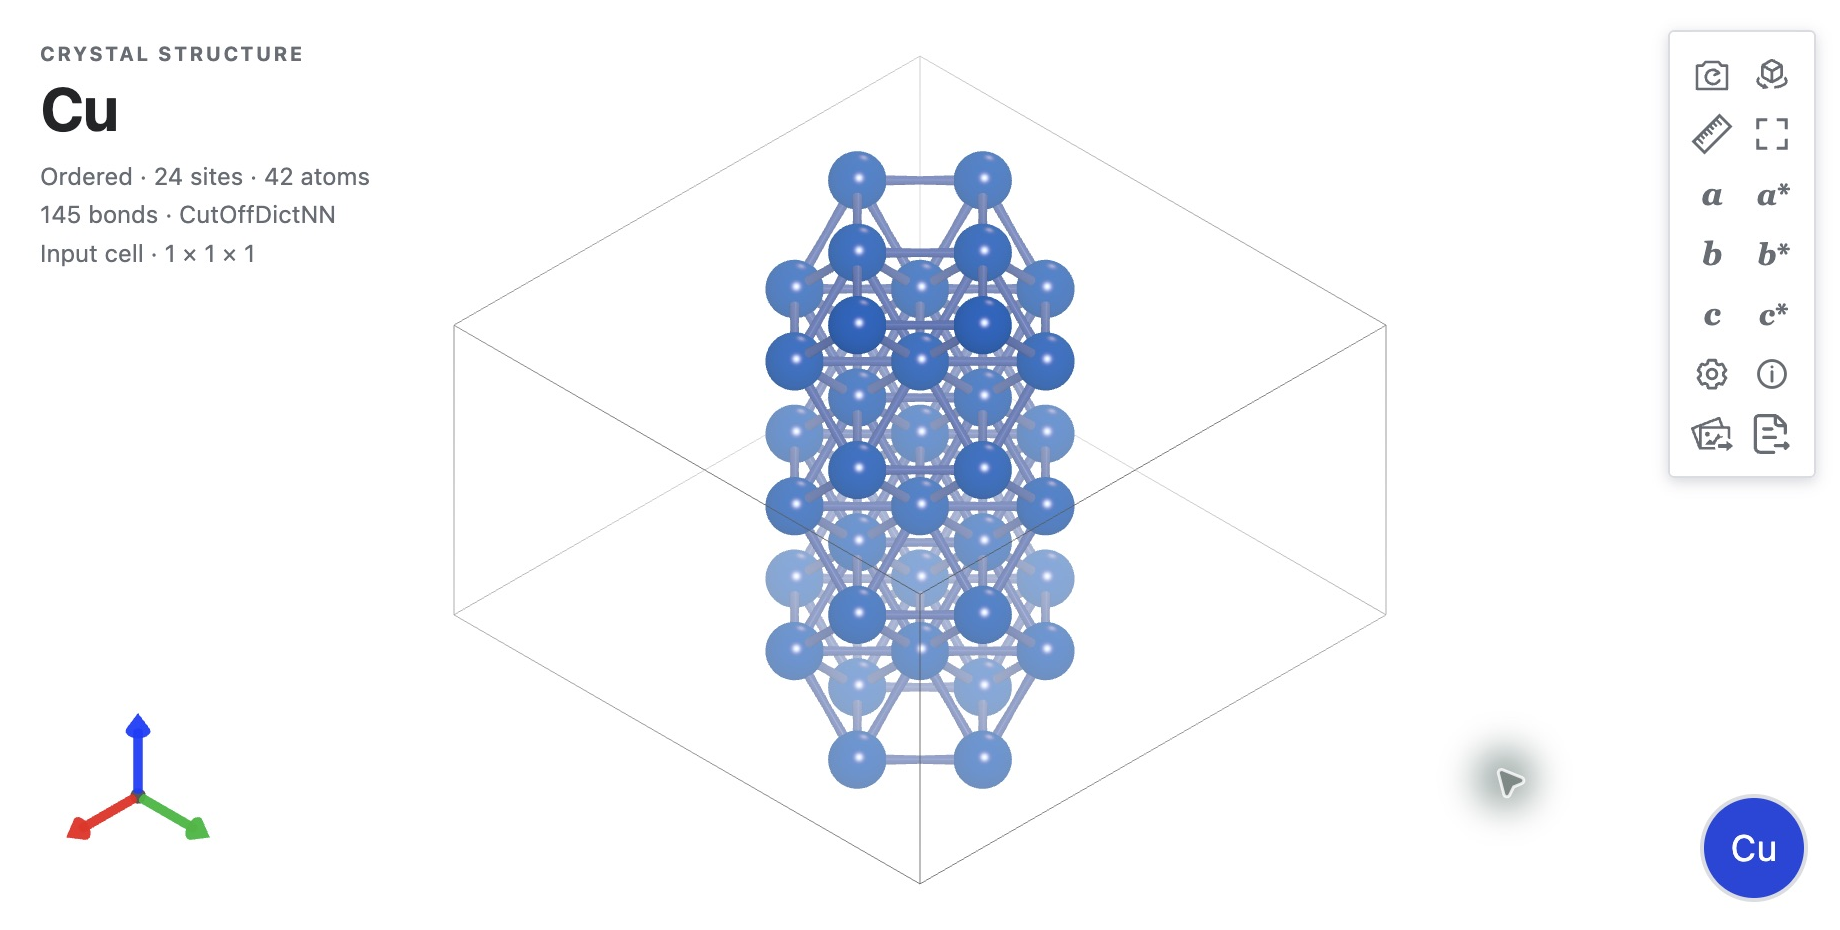
\includegraphics[width=\linewidth]{publication-assets/revision-nanowire-perspective.png}
\caption{The supplied 24-site copper nanowire in the viewer. Periodic boundary atoms show axial connectivity; transverse empty space is vacuum.}
\label{fig:nanowire-live}
\end{figure}

\FloatBarrier
\subsection{Inspect the wire's cross-section and axis}

Open \file{Cu-wire-001-r3-l2.json} to inspect the completed 24-site wire. Like the nanotube, it is periodic along $c$. The nanotube is made by rolling a sheet into a hollow cylinder; the copper wire retains crystal atoms inside a cylinder, including atoms within the cross-section.

\begin{steps}
  \item Import the JSON, open the document, and retain \ui{Input cell}. Check for Cu and 24 independent sites.
  \item Click \ui{c} to view down the axis. Discrete lattice positions may give a stepped outline rather than a smooth circle.
  \item Click \ui{a} or \ui{b} for a side view and show \ui{Unit cell}. The $7.22\,\text{\AA}$ axial length is the repeat period; the $13.415\,\text{\AA}$ transverse lengths accommodate the finite cross-section and vacuum.
  \item Clear unrelated selections and rotate slightly to show both end and side. Retain the cell boundary and orientation markers, and check that the view does not crop any atoms.
  \item If useful, set \ui{Repeat cell}'s \ui{c} to 2 to inspect connections, then restore one period. Save the project and structure. Record $[001]$, input radius $3\,\text{\AA}$, and 24 sites in exported figure captions.
\end{steps}

The input radius selects lattice positions; the retained discrete positions determine the actual outer span. The transverse span of $5.415\,\text{\AA}$ is smaller than diameter $6\,\text{\AA}$, consistent with the cut. Continue with suitable workflows for relaxation and electronic properties.

\subsection{Cut a finite copper cluster}
\index{Quantum dots}

The \ui{Quantum Dot} mode of \ui{Quantum Dot / Nano Void} retains atoms inside a sphere and makes the result nonperiodic in all three directions. This 13-site Cu cluster illustrates finite boundaries versus periodic bulk, and can be saved for subsequent electronic structure calculations.

\begin{steps}
  \item Reactivate the four-site copper input and open \ui{Quantum Dot / Nano Void} under \ui{Nanostructures}.
  \item Choose \ui{Quantum Dot}, radius $3\,\text{\AA}$, vacuum $4\,\text{\AA}$, and maximum atom count 2000.
  \item Preview and rotate the model. Check that no direction continues as an infinite atomic chain and that there are 13 Cu sites.
  \item Apply, name it \file{Cu-dot-r3}, and save the project and structure.
\end{steps}

All three cell lengths are approximately $11.61\,\text{\AA}$, while atoms span $3.61\,\text{\AA}$ in each direction. All periodicity flags are false. The shortest distance is approximately $2.552655\,\text{\AA}$. Using a $2.8\,\text{\AA}$ neighbor cutoff gives the central atom 12 neighbors and each of the 12 surface atoms 5. This initial cluster is cut directly from the face-centered cubic arrangement; its stable geometry requires optimization.

\subsection{Cut a spherical void in periodic copper}
\index{Nano voids}

Void mode retains the host outside the sphere and preserves the periodic box, the opposite of quantum-dot mode. Build a sufficiently large host first so that a small cell is not mostly or entirely removed.

\begin{steps}
  \item Import \file{Cu-void-host-2x2x2.json}, or use \ui{Build Supercell} on four-site Cu to make a $2\times2\times2$ host. Check for 32 Cu sites and cell lengths $7.22\,\text{\AA}$.
  \item Activate this host, open \ui{Quantum Dot / Nano Void}, choose \ui{Nano Void}, and set radius to $2.7\,\text{\AA}$. No external vacuum is needed around this periodic host.
  \item Preview with cell boundaries shown. The void center is fixed at host fractional position \((0.5,0.5,0.5)\). Check that central atoms are removed while the outer periodic host remains.
  \item Check that 13 atoms are removed, leaving 19 Cu sites. The cubic lattice remains $7.22\,\text{\AA}$ and periodic in all directions.
  \item Apply and save as \file{Cu-void-r2p7}, retaining the complete 32-site host for later radius changes or defect comparisons.
\end{steps}

The shortest periodic distance from the void center to a remaining atom is $3.61\,\text{\AA}$, larger than the input radius $2.7\,\text{\AA}$. This reflects discrete available lattice positions, not a failed radius setting. The host's shortest interatomic distance remains approximately $2.552655\,\text{\AA}$. Recording both the deletion-sphere radius and the closest remaining center-to-atom distance is clearer than a perspective view alone.

\subsection{Check periodicity and save the files}

Each native JSON retains its lattice, coordinates, periodicity flags, and construction metadata. CIF is used to exchange cell and atomic geometry, but these CIFs are imported as periodic in all directions. Use JSON to retain the low-dimensional periodicity in further modeling.

\begin{table}[htbp]
\centering\small
\caption{Site counts and native periodicity of the supplied nanostructures.}
\begin{tabularx}{\linewidth}{lX}
\toprule
Result & Model and key checks\\
\midrule
Graphene ribbon & 24C; periodic only in $y$; axial length $8.521690\,\text{\AA}$.\\
$(4,0)$ nanotube & 32C; periodic only in $z$; radius $1.566085\,\text{\AA}$.\\
Copper wire & 24Cu; periodic only in $z$; axial length $7.22\,\text{\AA}$.\\
Copper cluster & 13Cu; nonperiodic in all directions; cell lengths $11.61\,\text{\AA}$.\\
Copper with a void & 19Cu; periodic in all directions; 13 removed from a 32-site host.\\
\bottomrule
\end{tabularx}
\end{table}

\begin{steps}
  \item Save the project, giving inputs and derived results distinct names.
  \item For separate model files, choose JSON through \ui{Export file}\,$\rightarrow$\,\ui{Structure file}. Save CIF separately for geometry exchange. Do not choose the scene-oriented \ui{Scene JSON}.
  \item Reopen saved structures and check site count, cell, and periodic directions, then neighbors at edges, seams, or spherical cut boundaries.
  \item To regenerate these models, start MATLAB\regmark{} with \file{-nojvm}, configure the toolbox path, and run \file{nano_examples.m} from the examples directory. \file{verify_nano_examples.m} checks existing structures.
\end{steps}

These unpassivated starting models can be passivated, relaxed, and used in electronic structure calculations according to the material and boundaries. Retain both construction and calculation parameters, and confirm that the workflow references the intended structure.


\section{Example: build polymer chains}
\index{Polymers}

\subsection{Understand repeat units}

Polymer construction begins with repeat units. Built-in units include PE, PP, PS, PEO, and PPO. A user unit additionally needs head and tail atoms and atoms to remove when connecting. These definitions determine how adjacent units join, so check monomer topology before saving a repeat unit.

A homopolymer uses one unit type, a block copolymer groups types into consecutive blocks, and a random copolymer generates a sequence from composition and random rules. Sequence and spatial conformation are separate parameters. The same PE/PP sequence can start extended, zigzag, or as a random coil. A seed makes the same random construction conditions reproducible.

\subsection{A \headinglatin{PEO--PPO--PEO} triblock}

\begin{steps}
  \item Activate a molecular document. On \ui{Molecule Modeling}, open \ui{Polymer Builder} in \ui{Soft Matter}, then choose \ui{Build Block Copolymer}.
  \item Enter \literalinput{PEO PPO PEO} under \ui{Block repeat units} and \literalinput{3 4 3} under \ui{Block lengths}, separating entries with spaces. Set complete block-superunit repetitions to 1 and chain count to 1.
  \item Set seed to 8, choose \ui{Extended} under \ui{Initial conformation}, and leave head/tail end groups at \file{none}.
  \item Inspect the estimated atom count, preview, and apply. Check for 10 repeat units: 6 PEO and 4 PPO.
  \item Inspect the overall sequence, then zoom in on both block boundaries. Save under a sequence-specific name such as \file{PEO3-PPO4-PEO3}.
\end{steps}

The supplied \file{PEO3-PPO4-PEO3.json} has composition $\mathrm{C_{24}H_{50}O_{10}}$, 84 atoms, and 83 bonds. Ten units form one chain with nine inter-unit connections. Although end groups are \file{none}, hydrogens still complete unsatisfied terminal valences; include them when checking the formula.

% Native English captures; see docs/provenance/english-edition-assets.json for source and crop metadata.
\begin{figure}[H]
\centering
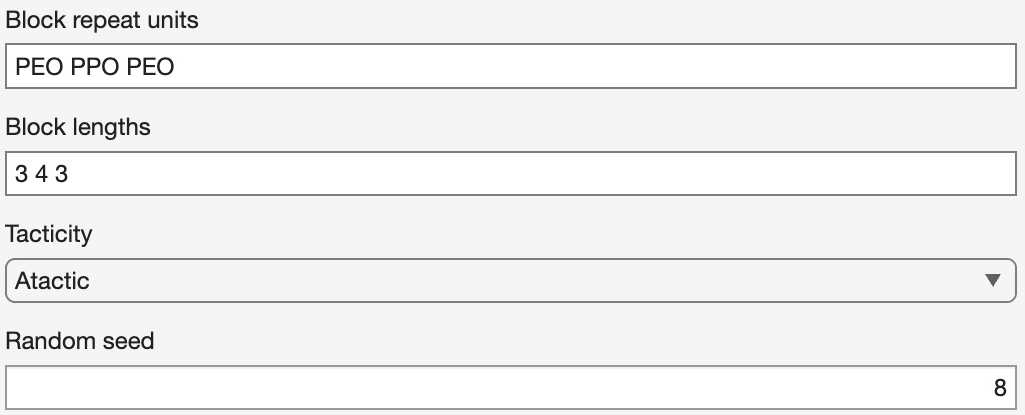
\includegraphics[width=\linewidth]{publication-assets/crop-3d7aab6f859860340b2f.png}
\par\vspace{3mm}
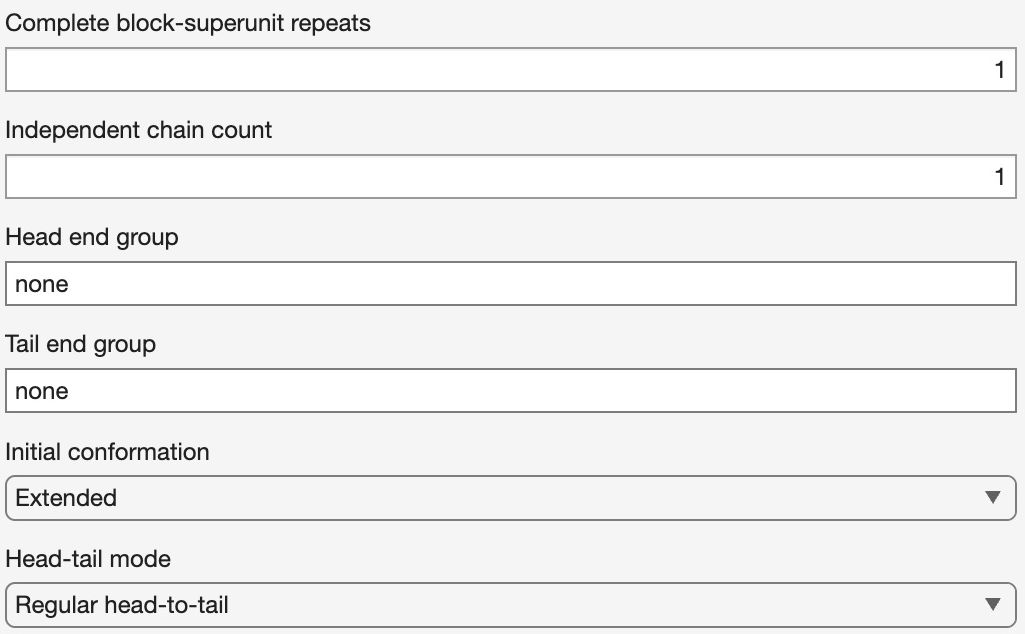
\includegraphics[width=\linewidth]{publication-assets/crop-14436d05d0623e7cdc6f.png}
\caption{Parameters for a PEO--PPO--PEO block chain. Above: \literalinput{PEO PPO PEO}, \literalinput{3 4 3}, and seed 8. Below: one repeat, one chain, both end groups \file{none}, an extended starting conformation, and regular head-to-tail connections.}
\label{fig:polymer-block-parameters}
\end{figure}

\begin{figure}[H]
\centering
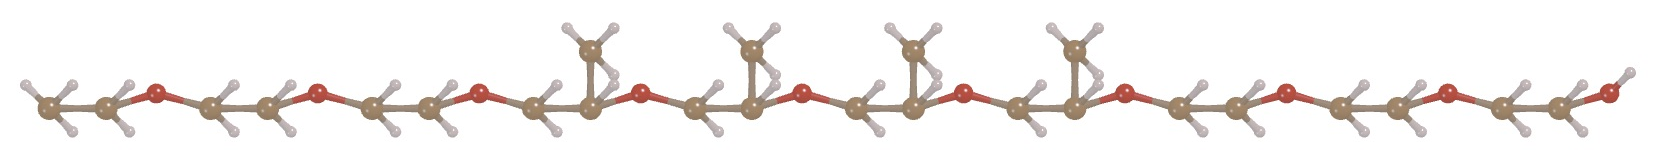
\includegraphics[width=\linewidth]{publication-assets/crop-7684a8a790954b6a1954.png}
\par\vspace{3mm}
\begin{minipage}[t]{40mm}
\vspace{0pt}
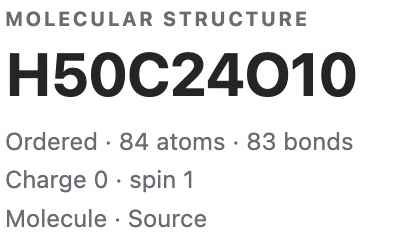
\includegraphics[width=\linewidth]{publication-assets/crop-c77f26280735587ce6a4.png}
\end{minipage}\hfill
\begin{minipage}[t]{80mm}
\vspace{0pt}
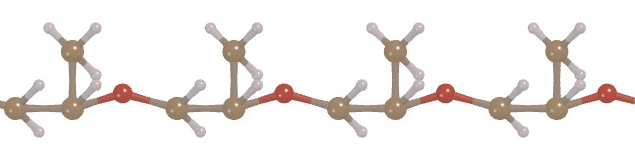
\includegraphics[width=\linewidth]{publication-assets/crop-71a6b6056b817444ef97.png}
\end{minipage}
\caption{The resulting initial block chain. Above: the complete chain. Below left: $\mathrm{C_{24}H_{50}O_{10}}$, 84 atoms, and 83 connections. Below right: the four methyl branches in the central PPO block.}
\label{fig:polymer-block-model}
\end{figure}


\subsection{A random chain with exact composition}

Create another molecular document and choose \ui{Build Random Copolymer}. Use PE and PP, mole fractions 0.3 and 0.7, 20 total repeats, exact composition enabled, and seed 91. The target is 6 PE and 14 PP units, with their sequence determined by the generation rules and seed.

Reactivity ratios control the terminal model for the random sequence. Retain \literalinput{1 1}, choose \ui{Extended} initial conformation and \ui{Syndiotactic} tacticity. The result should be $\mathrm{C_{54}H_{110}}$ with 164 atoms and 163 bonds, supplied as \file{PE6-PP14-seed91.json}. Its key difference from the block chain is unit order, not its filename or overall outline.

\ui{Tacticity} offers \ui{Syndiotactic}, \ui{Isotactic}, and \ui{Atactic}. The tool records the chosen flag. With the same seed, the syndiotactic and isotactic choices for this parameter set generate identical coordinates. This example checks exact composition, sequence, and connectivity. For tacticity studies, also verify the actual spatial arrangement of side groups.

Branched polymers specify a backbone unit, side-chain fragment, and attachment interval. Basic dendrimers specify generation, core functionality, and branching factor. Atom count grows rapidly with generation. Check estimated size before construction, verify connectivity in a small model, then scale up.

\section{Pack molecular mixtures}
\index{Mixture packing}

\subsection{Density and molecule counts}

Packing places molecules in a region while satisfying geometric constraints such as minimum contact distances. It is not a chemical reaction or molecular-dynamics equilibration. Target density is generally entered in $\mathrm{g/cm^3}$ and minimum contact distance in \AA. Higher density leaves less space and makes packing more difficult.

\ui{Construct Amorphous Cell} uses the current molecule as its component, with a molecule count, target density, contact distance, and seed. Begin with fewer molecules, check molecular integrity and box dimensions, then increase the count. Different components need not produce equal box sizes for the same molecule count, because molecular mass also enters the density relation.

\ui{Pack Mixture} uses the current molecule and a second project molecule. Specify composition by count, mole fraction, or mass fraction. Choose \ui{Exact counts} under \ui{Composition mode} and enter \literalinput{10 10} under \ui{Component counts} for ten molecules of each component. Fraction modes also require a total molecule count. Mole and mass fractions generally give different counts for components of different molecular masses; check the actual counts in the result report.

\subsection{Exercise: pack ten water and ten ethanol molecules}

Import \file{water-packing.json} and \file{ethanol-optimized.json}. The former retains water's two O--H bonds; the latter is the optimized ethanol from Chapter~\ref{ch:modeling}. Activate water, open \ui{Pack Mixture}, and choose ethanol under \ui{Second project molecule}.

Choose \ui{Exact counts}, enter \literalinput{10 10}, and set density to $0.1\,\mathrm{g/cm^3}$, tolerance to $1.2\,\text{\AA}$, and seed to 23. Retain 100 molecules per batch and leave density ramp stages blank. The low initial density makes molecular integrity easy to inspect. The equilibrium density of the liquid mixture is determined during subsequent equilibration.

The result, \file{water10-ethanol10-packed.json}, has 20 molecules, 120 atoms, and composition $\mathrm{C_{20}H_{80}O_{20}}$. Its cubic side length is approximately $21.9954\,\text{\AA}$; total mass divided by volume gives $0.1\,\mathrm{g/cm^3}$. The shortest intermolecular distance, including periodic images, is approximately $4.0990\,\text{\AA}$, while intramolecular distances remain unchanged. Contact requirements apply between molecules, not to water's internal O--H bonds.

Retain both component inputs when saving the result. The packed structure records molecule and component indices but not a complete global explicit bond table. Further topology work therefore still needs the original component connectivity. The accompanying \file{interface_packing_examples.m} provides component inputs, candidate structures, and contact checks.

\subsection{Choose the packing region}

\ui{Build Confined Layer} adds a confinement axis and allowed region, concentrating molecules in part of the box. Check whether bounds are fractional or dimensional and match them to the selected axis. \ui{Pack into Existing Box} retains the host and adds project molecules to its cell. \ui{Pack around Nanoparticle} additionally specifies a gap around the host to avoid placing molecules directly against its surface.

For packing failures, adjust the geometry: lower the initial density or molecule count, enlarge the region, reconsider the contact distance, or try another seed. Optional density ramps and batch packing help control larger jobs. Check composition, cross-boundary contacts, and unresolved issues in the report before minimization, thermal treatment, or equilibration suited to your study.

\begin{notebox}{Save reproducible models}
For polymer and packed models, retain the repeat units or components, counts and density, seed, conformation, contact requirements, and generated structure together. A seed alone does not identify the model's origin. Saving these conditions with the project makes rebuilding and comparison much easier.
\end{notebox}
